\documentclass[11pt, letterpaper]{article}

% Fonts and Encoding
\usepackage[utf8]{inputenc}
\usepackage[T1]{fontenc}
\usepackage{lmodern} % High-quality Latin Modern vector font

% Math and Symbols
\usepackage{amsmath, amssymb, amsthm, amsfonts, mathrsfs, mathtools}

% Layout and Geometry
\usepackage{geometry}
\geometry{letterpaper, margin=1in}
\setlength{\parindent}{0pt}
\setlength{\parskip}{0.6em}

% Formatting and Graphics
\usepackage{graphicx, xcolor, enumitem, booktabs, array, tabularx}

% TikZ for Illustrations
\usepackage{tikz}
\usetikzlibrary{arrows.meta, positioning, shapes.geometric, calc, backgrounds, matrix}

% Clickable Links and TOC
\usepackage{hyperref}
\hypersetup{
    colorlinks=true,
    linkcolor=blue,
    filecolor=magenta,      
    urlcolor=cyan,
    pdftitle={Inner Product Spaces: Comprehensive Mastery Guide},
}

% Theorem Environments
\newtheorem{theorem}{Theorem}[section]
\newtheorem{lemma}[theorem]{Lemma}
\newtheorem{proposition}[theorem]{Proposition}
\newtheorem{corollary}[theorem]{Corollary}
\theoremstyle{definition}
\newtheorem{definition}{Definition}[section]
\newtheorem{axiom}{Axiom}[section]
\newtheorem{example}{Example}[section]
\theoremstyle{remark}
\newtheorem{remark}{Remark}[section]

% Custom Commands (Enforced standard notation)
\newcommand{\R}{\mathbb{R}}
\newcommand{\N}{\mathbb{N}}
\newcommand{\Z}{\mathbb{Z}}
\newcommand{\Q}{\mathbb{Q}}
\newcommand{\E}{\mathbb{E}}
\newcommand{\Prob}{\mathbb{P}}
\newcommand{\F}{\mathcal{F}}

\title{Inner Product Spaces: Comprehensive Mastery Guide\\(Section 6.7)}
\author{Tashfeen Omran}
\date{\today}

\begin{document}

\maketitle
\tableofcontents
\newpage

\section{Comprehensive Introduction, Context, and Prerequisites}

\subsection{Core Concepts}

In Euclidean space $\mathbb{R}^n$, the standard dot product $\mathbf{u} \cdot \mathbf{v} = u_1 v_1 + \cdots + u_n v_n$ gives us a complete geometric toolkit: we can measure the length of a vector, compute the distance between two vectors, test whether two vectors are perpendicular, and project a vector orthogonally onto a subspace to solve best-approximation (least-squares) problems. However, many fundamental mathematical objects—such as polynomials in $\mathbb{P}_n$, continuous functions in $C[a, b]$, or signals sampled at discrete nodes—form vector spaces that are not literally $\mathbb{R}^n$.

To import the geometry of $\mathbb{R}^n$ into general real vector spaces, we replace the coordinate-specific formula of the dot product with an abstract function satisfying the four algebraic properties that make Euclidean geometry work.

\begin{definition}[Inner Product and Inner Product Space]
An \textbf{inner product} on a real vector space $V$ is a function that, to each pair of vectors $\mathbf{u}$ and $\mathbf{v}$ in $V$, associates a real number $\langle \mathbf{u}, \mathbf{v} \rangle$ satisfying the following four axioms for all $\mathbf{u}, \mathbf{v}, \mathbf{w} \in V$ and all scalars $c \in \mathbb{R}$:
\begin{enumerate}[label=\textbf{\arabic*.}]
    \item \textbf{Symmetry:} $\langle \mathbf{u}, \mathbf{v} \rangle = \langle \mathbf{v}, \mathbf{u} \rangle$.
    \item \textbf{Additivity:} $\langle \mathbf{u} + \mathbf{v}, \mathbf{w} \rangle = \langle \mathbf{u}, \mathbf{w} \rangle + \langle \mathbf{v}, \mathbf{w} \rangle$.
    \item \textbf{Homogeneity:} $\langle c\mathbf{u}, \mathbf{v} \rangle = c \langle \mathbf{u}, \mathbf{v} \rangle$.
    \item \textbf{Positive-Definiteness:} $\langle \mathbf{u}, \mathbf{u} \rangle \ge 0$, and $\langle \mathbf{u}, \mathbf{u} \rangle = 0$ if and only if $\mathbf{u} = \mathbf{0}$.
\end{enumerate}
A vector space $V$ equipped with an inner product is called an \textbf{inner product space}.
\end{definition}

Once an inner product $\langle \cdot, \cdot \rangle$ is fixed on $V$, every geometric notion from $\mathbb{R}^n$ carries over verbatim:
\begin{itemize}
    \item \textbf{Length (Norm):} The norm of $\mathbf{v} \in V$ is $\|\mathbf{v}\| = \sqrt{\langle \mathbf{v}, \mathbf{v} \rangle}$, or equivalently $\|\mathbf{v}\|^2 = \langle \mathbf{v}, \mathbf{v} \rangle$. This is well-defined because $\langle \mathbf{v}, \mathbf{v} \rangle \ge 0$ by Axiom 4.
    \item \textbf{Unit Vector:} A vector $\mathbf{u} \in V$ is a unit vector if $\|\mathbf{u}\| = 1$ (equivalently, $\langle \mathbf{u}, \mathbf{u} \rangle = 1$).
    \item \textbf{Distance:} The distance between $\mathbf{u}$ and $\mathbf{v}$ is $\operatorname{dist}(\mathbf{u}, \mathbf{v}) = \|\mathbf{u} - \mathbf{v}\|$.
    \item \textbf{Orthogonality:} Vectors $\mathbf{u}$ and $\mathbf{v}$ are orthogonal if $\langle \mathbf{u}, \mathbf{v} \rangle = 0$.
    \item \textbf{Orthogonal Projection and Best Approximation:} If $W$ is a finite-dimensional subspace of $V$ with an orthogonal basis $\{\mathbf{w}_1, \dots, \mathbf{w}_p\}$, then the unique vector in $W$ closest to $\mathbf{v} \in V$ (minimizing $\|\mathbf{v} - \mathbf{w}\|$ over all $\mathbf{w} \in W$) is the orthogonal projection:
    \[
        \operatorname{proj}_W \mathbf{v} = \frac{\langle \mathbf{v}, \mathbf{w}_1 \rangle}{\langle \mathbf{w}_1, \mathbf{w}_1 \rangle}\mathbf{w}_1 + \frac{\langle \mathbf{v}, \mathbf{w}_2 \rangle}{\langle \mathbf{w}_2, \mathbf{w}_2 \rangle}\mathbf{w}_2 + \cdots + \frac{\langle \mathbf{v}, \mathbf{w}_p \rangle}{\langle \mathbf{w}_p, \mathbf{w}_p \rangle}\mathbf{w}_p.
    \]
    \item \textbf{The Gram--Schmidt Process:} Given any basis $\{\mathbf{x}_1, \dots, \mathbf{x}_p\}$ of a finite-dimensional subspace $W \subseteq V$, we recursively construct an orthogonal basis $\{\mathbf{v}_1, \dots, \mathbf{v}_p\}$ by setting $\mathbf{v}_1 = \mathbf{x}_1$ and
    \[
        \mathbf{v}_k = \mathbf{x}_k - \sum_{j=1}^{k-1} \frac{\langle \mathbf{x}_k, \mathbf{v}_j \rangle}{\langle \mathbf{v}_j, \mathbf{v}_j \rangle}\mathbf{v}_j \quad \text{for } k = 2, \dots, p.
    \]
\end{itemize}

Crucially, the textbook introduces three canonical families of inner products beyond the standard dot product:
\begin{enumerate}
    \item \textbf{Weighted Inner Products on $\mathbb{R}^n$:} For fixed positive weights $c_1, \dots, c_n > 0$,
    \[
        \langle \mathbf{u}, \mathbf{v} \rangle = c_1 u_1 v_1 + c_2 u_2 v_2 + \cdots + c_n u_n v_n.
    \]
    \item \textbf{Evaluation Inner Products on $\mathbb{P}_n$:} For $n+1$ distinct real nodes $t_0, t_1, \dots, t_n$,
    \[
        \langle p, q \rangle = p(t_0)q(t_0) + p(t_1)q(t_1) + \cdots + p(t_n)q(t_n).
    \]
    Axiom 4 holds because a nonzero polynomial of degree at most $n$ can vanish at most $n$ times; hence vanishing at $n+1$ distinct points forces $p$ to be the zero polynomial.
    \item \textbf{Integral Inner Products on $C[a, b]$:} For continuous functions $f, g \in C[a, b]$,
    \[
        \langle f, g \rangle = \int_a^b f(t)g(t)\,dt.
    \]
    Axiom 4 holds because $[f(t)]^2 \ge 0$ is continuous on $[a, b]$, so $\int_a^b [f(t)]^2\,dt = 0$ forces $[f(t)]^2 \equiv 0$, i.e., $f$ is the zero function on $[a, b]$.
\end{enumerate}

\subsection{Intuition and Derivation}

\subsubsection*{Why the Two Fundamental Inequalities Hold}
In any inner product space $V$, let $\mathbf{u}, \mathbf{v} \in V$. If $\mathbf{u} \ne \mathbf{0}$, let $W = \operatorname{Span}\{\mathbf{u}\}$. Splitting $\mathbf{v}$ into its projection $\operatorname{proj}_W \mathbf{v}$ onto $W$ and its orthogonal residual $\mathbf{v} - \operatorname{proj}_W \mathbf{v}$ yields a right triangle in $V$:
\[
    \langle \operatorname{proj}_W \mathbf{v}, \, \mathbf{v} - \operatorname{proj}_W \mathbf{v} \rangle = 0.
\]
Expanding $\|\mathbf{v}\|^2 = \|\operatorname{proj}_W \mathbf{v} + (\mathbf{v} - \operatorname{proj}_W \mathbf{v})\|^2$ using Axioms 1--3 gives the abstract **Pythagorean Theorem**:
\[
    \|\mathbf{v}\|^2 = \|\operatorname{proj}_W \mathbf{v}\|^2 + \|\mathbf{v} - \operatorname{proj}_W \mathbf{v}\|^2 \ge \|\operatorname{proj}_W \mathbf{v}\|^2.
\]
Since $\|\operatorname{proj}_W \mathbf{v}\| = \left\| \frac{\langle \mathbf{v}, \mathbf{u} \rangle}{\langle \mathbf{u}, \mathbf{u} \rangle}\mathbf{u} \right\| = \frac{|\langle \mathbf{u}, \mathbf{v} \rangle|}{\|\mathbf{u}\|^2}\|\mathbf{u}\| = \frac{|\langle \mathbf{u}, \mathbf{v} \rangle|}{\|\mathbf{u}\|}$, the inequality $\|\operatorname{proj}_W \mathbf{v}\| \le \|\mathbf{v}\|$ immediately yields the **Cauchy--Schwarz Inequality**:
\[
    |\langle \mathbf{u}, \mathbf{v} \rangle| \le \|\mathbf{u}\|\,\|\mathbf{v}\|.
\]
In turn, Cauchy--Schwarz gives the **Triangle Inequality** by expanding $\|\mathbf{u} + \mathbf{v}\|^2$:
\[
    \|\mathbf{u} + \mathbf{v}\|^2 = \|\mathbf{u}\|^2 + 2\langle \mathbf{u}, \mathbf{v} \rangle + \|\mathbf{v}\|^2 \le \|\mathbf{u}\|^2 + 2|\langle \mathbf{u}, \mathbf{v} \rangle| + \|\mathbf{v}\|^2 \le \|\mathbf{u}\|^2 + 2\|\mathbf{u}\|\,\|\mathbf{v}\| + \|\mathbf{v}\|^2 = (\|\mathbf{u}\| + \|\mathbf{v}\|)^2.
\]
Taking nonnegative square roots gives $\|\mathbf{u} + \mathbf{v}\| \le \|\mathbf{u}\| + \|\mathbf{v}\|$.

\begin{figure}[htbp]
\centering
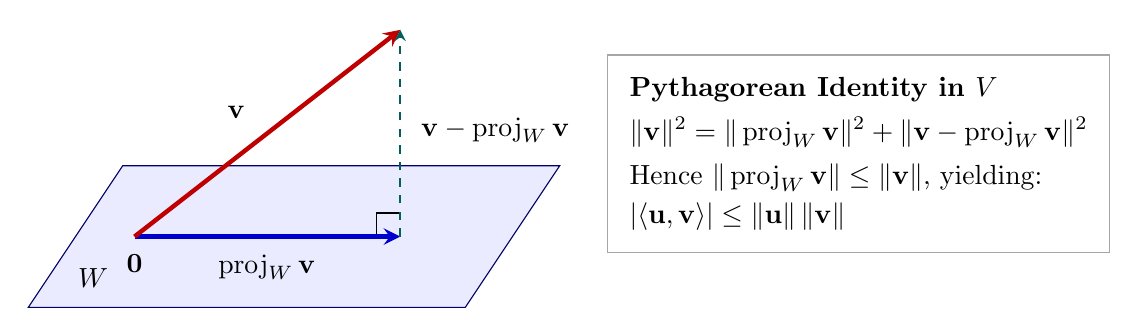
\begin{tikzpicture}[scale=1.5]
    % Layer 1: Background plane W
    \fill[blue!8] (-0.3,-0.4) -- (3.4,-0.4) -- (4.2,0.8) -- (0.5,0.8) -- cycle;
    % Layer 2: Plane boundary and right-angle symbol
    \draw[thin, blue!40!black] (-0.3,-0.4) -- (3.4,-0.4) -- (4.2,0.8) -- (0.5,0.8) -- cycle;
    \draw[thin, black] (2.65,0.20) -- (2.65,0.40) -- (2.85,0.40);
    % Layer 3: Vectors and orthogonal residual
    \draw[->, >=stealth, ultra thick, blue!80!black] (0.6,0.2) -- (2.85,0.2);
    \draw[->, >=stealth, ultra thick, red!75!black] (0.6,0.2) -- (2.85,1.95);
    \draw[->, >=stealth, thick, dashed, teal!75!black] (2.85,0.2) -- (2.85,1.95);
    % Layer 4: Labels and single-node annotation
    \node[black, below=3pt] at (0.6,0.2) {$\mathbf{0}$};
    \node[black, below=3pt] at (1.72,0.2) {$\operatorname{proj}_W \mathbf{v}$};
    \node[black, above left=2pt] at (1.65,1.08) {$\mathbf{v}$};
    \node[black, right=4pt] at (2.85,1.10) {$\mathbf{v} - \operatorname{proj}_W \mathbf{v}$};
    \node[black] at (0.25,-0.15) {$W$};
    \node[align=left, inner sep=8pt, draw=black!35, fill=white, anchor=west, text=black] at (4.6, 0.9) {
        \textbf{Pythagorean Identity in $V$}\\[4pt]
        $\displaystyle \|\mathbf{v}\|^2 = \|\operatorname{proj}_W \mathbf{v}\|^2 + \|\mathbf{v} - \operatorname{proj}_W \mathbf{v}\|^2$\\[4pt]
        Hence $\displaystyle \|\operatorname{proj}_W \mathbf{v}\| \le \|\mathbf{v}\|$, yielding:\\[2pt]
        $\displaystyle |\langle \mathbf{u}, \mathbf{v} \rangle| \le \|\mathbf{u}\|\,\|\mathbf{v}\|$
    };
\end{tikzpicture}
\caption{Orthogonal decomposition of $\mathbf{v}$ onto a finite-dimensional subspace $W$ and the geometric origin of the Cauchy--Schwarz inequality.}
\end{figure}

\subsubsection*{Deriving the Integral Inner Product from Evaluation Inner Products}
Why is $\int_a^b f(t)g(t)\,dt$ the natural continuous analogue of the dot product? Suppose $p, q$ are polynomials on $[a, b]$, and pick $n$ larger than or equal to the degrees of $p$ and $q$. Partition $[a, b]$ into $n+1$ subintervals of equal width $\Delta t = \frac{b-a}{n+1}$, and choose a sample node $t_j$ in each subinterval ($j = 0, 1, \dots, n$). Because the raw sum $\sum_{j=0}^n p(t_j)q(t_j)$ grows arbitrarily large as $n \to \infty$, we normalize by dividing by $n+1$. Using $\frac{1}{n+1} = \frac{\Delta t}{b-a}$, we obtain
\[
    \frac{1}{n+1} \sum_{j=0}^n p(t_j)q(t_j) = \frac{1}{b-a} \left[ \sum_{j=0}^n p(t_j)q(t_j)\,\Delta t \right].
\]
The bracketed sum is a Riemann sum for $p(t)q(t)$ on $[a, b]$. Letting $n \to \infty$ gives the average product $\frac{1}{b-a}\int_a^b p(t)q(t)\,dt$. Dropping the positive constant factor $\frac{1}{b-a}$ (which leaves orthogonality and all four axioms unchanged) yields $\langle f, g \rangle = \int_a^b f(t)g(t)\,dt$ for all $f, g \in C[a, b]$.

\begin{figure}[htbp]
\centering
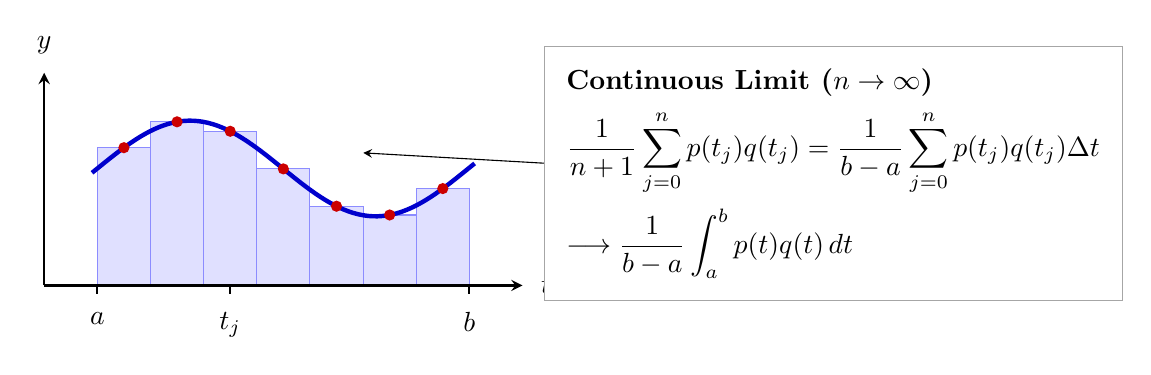
\begin{tikzpicture}[scale=1.35]
    % Layer 1: Riemann rectangles under p(t)q(t)
    \foreach \x in {0.5, 1.0, 1.5, 2.0, 2.5, 3.0, 3.5} {
        \pgfmathsetmacro{\mid}{\x + 0.25}
        \pgfmathsetmacro{\h}{1.1 + 0.45*sin(deg(1.8*(\mid - 0.5)))}
        \fill[blue!12] (\x, 0) rectangle (\x+0.5, \h);
        \draw[blue!45] (\x, 0) rectangle (\x+0.5, \h);
    }
    % Layer 2: Axes and explicit tick marks
    \draw[->, >=stealth, thick, black] (0,0) -- (4.5,0) node[right=3pt, black] {$t$};
    \draw[->, >=stealth, thick, black] (0,0) -- (0,2.0) node[above=3pt, black] {$y$};
    \draw[thick] (0.5,0) -- (0.5,-0.08) node[below=3pt, black] {$a$};
    \draw[thick] (4.0,0) -- (4.0,-0.08) node[below=3pt, black] {$b$};
    \draw[thick] (1.75,0) -- (1.75,-0.08) node[below=3pt, black] {$t_j$};
    % Layer 3: Continuous product curve and sample dots
    \draw[ultra thick, blue!80!black, domain=0.45:4.05, samples=80] plot (\x, {1.1 + 0.45*sin(deg(1.8*(\x - 0.5)))});
    \foreach \x in {0.5, 1.0, 1.5, 2.0, 2.5, 3.0, 3.5} {
        \pgfmathsetmacro{\mid}{\x + 0.25}
        \pgfmathsetmacro{\h}{1.1 + 0.45*sin(deg(1.8*(\mid - 0.5)))}
        \fill[red!80!black] (\mid, \h) circle (1.5pt);
    }
    % Layer 4: Off-axis callout and annotation box
    \draw[->, >=stealth, shorten >=2pt, black] (4.7, 1.15) -- (2.95, 1.25);
    \node[align=left, inner sep=8pt, draw=black!35, fill=white, anchor=west, text=black] at (4.7, 1.05) {
        \textbf{Continuous Limit ($n \to \infty$)}\\[4pt]
        $\displaystyle \frac{1}{n+1}\sum_{j=0}^n p(t_j)q(t_j) = \frac{1}{b-a}\sum_{j=0}^n p(t_j)q(t_j)\Delta t$\\[4pt]
        $\displaystyle \longrightarrow \frac{1}{b-a}\int_a^b p(t)q(t)\,dt$
    };
\end{tikzpicture}
\caption{Passing from discrete evaluation inner products on $\mathbb{P}_n$ to the integral inner product on $C[a, b]$ via Riemann sums.}
\end{figure}

\subsection{Historical Context and Motivation}

The axiomatic theory of inner product spaces grew out of a profound convergence of eighteenth- and nineteenth-century analysis, approximation theory, and mathematical physics. In 1807--1822, Jean-Baptiste Joseph Fourier modeled heat conduction by decomposing arbitrary temperature profiles into infinite sums of sines and cosines, discovering empirically that the coefficients could be isolated via definite integrals of products—what we now recognize as orthogonal projection in $C[-\pi, \pi]$. Earlier, Adrien-Marie Legendre (1782) had introduced his orthogonal polynomials while computing gravitational potentials of ellipsoids, and Pafnuty Chebyshev later generalized discrete and weighted orthogonal polynomials to minimize approximation errors in mechanical linkages.

The formal tools binding these disparate settings emerged over the nineteenth and early twentieth centuries. Augustin-Louis Cauchy established the finite-sum inequality in 1821, Viktor Bunyakovsky extended it to integrals in 1859, and Hermann Schwarz proved the general integral version in 1885 while studying minimal surfaces. Finally, David Hilbert (1904--1910) and Erhard Schmidt (1907--1908) unified sequences ($\ell^2$), continuous functions ($L^2[a,b]$), and Euclidean vectors ($\mathbb{R}^n$) under a single geometric framework—introducing the Gram--Schmidt orthogonalization procedure and the modern axiomatic view of inner product spaces.

\subsection{Key Formulas}

\renewcommand{\arraystretch}{1.5}
\begin{tabularx}{\textwidth}{>{\raggedright\arraybackslash}p{4.3cm} >{$\displaystyle}c<{$} X}
\toprule
\textbf{Concept} & \textbf{Formula} & \textbf{Meaning and Usage} \\
\midrule
Weighted Inner Product ($\mathbb{R}^n$) & \langle \mathbf{u}, \mathbf{v} \rangle = \sum_{i=1}^n w_i u_i v_i & Requires all weights $w_i > 0$ so Axiom 4 holds. \\
\addlinespace[4pt]
Evaluation Inner Product ($\mathbb{P}_n$) & \langle p, q \rangle = \sum_{j=0}^n p(t_j)q(t_j) & Requires $n+1$ distinct nodes $t_0, \dots, t_n$; isomorphic to dot product on $\mathbb{R}^{n+1}$. \\
\addlinespace[4pt]
Integral Inner Product ($C[a,b]$) & \langle f, g \rangle = \int_a^b f(t)g(t)\,dt & Standard continuous inner product for function approximation and Fourier analysis. \\
\addlinespace[4pt]
Norm and Distance & \|\mathbf{v}\| = \sqrt{\langle \mathbf{v}, \mathbf{v} \rangle}, \quad d(\mathbf{u}, \mathbf{v}) = \|\mathbf{u} - \mathbf{v}\| & Measures vector length and closeness between vectors or functions. \\
\addlinespace[4pt]
Orthogonal Projection & \operatorname{proj}_W \mathbf{v} = \sum_{i=1}^p \frac{\langle \mathbf{v}, \mathbf{w}_i \rangle}{\langle \mathbf{w}_i, \mathbf{w}_i \rangle}\mathbf{w}_i & Best approximation to $\mathbf{v}$ in $W$ when $\{\mathbf{w}_1, \dots, \mathbf{w}_p\}$ is an orthogonal basis of $W$. \\
\addlinespace[4pt]
Cauchy--Schwarz Inequality & |\langle \mathbf{u}, \mathbf{v} \rangle| \le \|\mathbf{u}\|\,\|\mathbf{v}\| & Bounds inner products by norms; equality holds iff $\mathbf{u}$ and $\mathbf{v}$ are linearly dependent. \\
\addlinespace[4pt]
Triangle Inequality & \|\mathbf{u} + \mathbf{v}\| \le \|\mathbf{u}\| + \|\mathbf{v}\| & Ensures distance satisfies the metric triangle property. \\
\bottomrule
\end{tabularx}

\subsection{Prerequisites}

To master Section 6.7 seamlessly, you must have complete command of the following prerequisites:
\begin{itemize}
    \item \textbf{Euclidean Geometry in $\mathbb{R}^n$ (Sections 6.1--6.4):} Standard dot products, orthogonality, orthogonal projections onto lines and subspaces, the Orthogonal Decomposition Theorem, the Best Approximation Theorem, and the Gram--Schmidt process in $\mathbb{R}^n$.
    \item \textbf{Vector Spaces and Linear Transformations (Chapter 4):} Vector space axioms, subspaces, linear independence, bases, coordinate vectors, and one-to-one (injective) linear transformations / isomorphisms.
    \item \textbf{Matrix Invertibility (Chapter 2):} Invertible Matrix Theorem ($A\mathbf{u} = \mathbf{0} \iff \mathbf{u} = \mathbf{0}$ for invertible $A$) and matrix transpose properties $(AB)^T = B^T A^T$.
    \item \textbf{Single-Variable Calculus:} Definite integration of polynomials and trigonometric functions, Riemann sums, parity rules ($\int_{-a}^a (\text{odd})\,dt = 0$), and the fact that a continuous nonnegative function with zero integral is identically zero.
    \item \textbf{Algebra and Trigonometry:} Root properties of polynomials (a degree-$n$ polynomial with $n+1$ roots is identically zero) and trigonometric power-reduction / triple-angle identities.
\end{itemize}

\newpage
\section{Detailed Homework Solutions}

For completeness, we begin with the two Practice Problems from the Section 6.7 text, followed by complete, step-by-step solutions to every single exercise (Exercises 1--34) in Section 6.7.

\subsection{Practice Problems}

\textbf{Practice Problem 1 (Original Problem):} Use the inner product axioms to verify that $\langle \mathbf{v}, \mathbf{0} \rangle = \langle \mathbf{0}, \mathbf{v} \rangle = 0$.

\textbf{Solution:}
\begin{enumerate}
    \item By Axiom 1 (symmetry), $\langle \mathbf{v}, \mathbf{0} \rangle = \langle \mathbf{0}, \mathbf{v} \rangle$.
    \item In any vector space, the zero vector satisfies $\mathbf{0} = 0\mathbf{v}$. Applying Axiom 3 (homogeneity) with scalar $c = 0$:
    \[
        \langle \mathbf{0}, \mathbf{v} \rangle = \langle 0\mathbf{v}, \mathbf{v} \rangle = 0\langle \mathbf{v}, \mathbf{v} \rangle = 0.
    \]
    \item Combining both steps gives $\langle \mathbf{v}, \mathbf{0} \rangle = \langle \mathbf{0}, \mathbf{v} \rangle = 0$. \hfill $\blacksquare$
\end{enumerate}

\textbf{Practice Problem 2 (Original Problem):} Use the inner product axioms to verify that $\langle \mathbf{u}, \mathbf{v} + \mathbf{w} \rangle = \langle \mathbf{u}, \mathbf{v} \rangle + \langle \mathbf{u}, \mathbf{w} \rangle$.

\textbf{Solution:}
Applying Axiom 1 (symmetry), then Axiom 2 (additivity in the first slot), and then Axiom 1 again to each resulting term:
\[
    \langle \mathbf{u}, \mathbf{v} + \mathbf{w} \rangle = \langle \mathbf{v} + \mathbf{w}, \mathbf{u} \rangle = \langle \mathbf{v}, \mathbf{u} \rangle + \langle \mathbf{w}, \mathbf{u} \rangle = \langle \mathbf{u}, \mathbf{v} \rangle + \langle \mathbf{u}, \mathbf{w} \rangle. \qquad \blacksquare
\]

\subsection{Exercises 1--2: Weighted Inner Products on $\mathbb{R}^2$}

\textbf{Exercise 1 (Original Problem):} Let $\mathbb{R}^2$ have the inner product of Example 1, and let $\mathbf{x} = (1, 1)$ and $\mathbf{y} = (5, -1)$.
\begin{enumerate}[label=\textbf{\alph*.}]
    \item Find $\|\mathbf{x}\|$, $\|\mathbf{y}\|$, and $|\langle \mathbf{x}, \mathbf{y} \rangle|^2$.
    \item Describe all vectors $(z_1, z_2)$ that are orthogonal to $\mathbf{y}$.
\end{enumerate}

\textbf{Solution:}
In Example 1, the inner product on $\mathbb{R}^2$ is $\langle \mathbf{u}, \mathbf{v} \rangle = 4u_1 v_1 + 5u_2 v_2$.
\begin{enumerate}[label=\textbf{\alph*.}]
    \item Compute each squared norm and then take square roots:
    \begin{align*}
        \|\mathbf{x}\|^2 &= \langle \mathbf{x}, \mathbf{x} \rangle = 4(1)(1) + 5(1)(1) = 4 + 5 = 9 \implies \|\mathbf{x}\| = \sqrt{9} = 3, \\
        \|\mathbf{y}\|^2 &= \langle \mathbf{y}, \mathbf{y} \rangle = 4(5)(5) + 5(-1)(-1) = 100 + 5 = 105 \implies \|\mathbf{y}\| = \sqrt{105}.
    \end{align*}
    Next, compute the inner product $\langle \mathbf{x}, \mathbf{y} \rangle$:
    \[
        \langle \mathbf{x}, \mathbf{y} \rangle = 4(1)(5) + 5(1)(-1) = 20 - 5 = 15,
    \]
    so
    \[
        |\langle \mathbf{x}, \mathbf{y} \rangle|^2 = |15|^2 = 225.
    \]
    \textbf{Final Answer (a):} $\|\mathbf{x}\| = 3$, $\|\mathbf{y}\| = \sqrt{105}$, and $|\langle \mathbf{x}, \mathbf{y} \rangle|^2 = 225$.

    \item A vector $\mathbf{z} = (z_1, z_2) \in \mathbb{R}^2$ is orthogonal to $\mathbf{y} = (5, -1)$ if and only if $\langle \mathbf{z}, \mathbf{y} \rangle = 0$:
    \[
        4z_1(5) + 5z_2(-1) = 0 \implies 20z_1 - 5z_2 = 0 \implies 5z_2 = 20z_1 \implies z_2 = 4z_1.
    \]
    Hence $\mathbf{z} = (z_1, 4z_1) = z_1(1, 4)$ for any $z_1 \in \mathbb{R}$.\\
    \textbf{Final Answer (b):} All vectors of the form $(z_1, 4z_1)$ for $z_1 \in \mathbb{R}$, i.e., $\operatorname{Span}\{(1, 4)\}$.
\end{enumerate}

\textbf{Exercise 2 (Original Problem):} Let $\mathbb{R}^2$ have the inner product of Example 1. Show that the Cauchy--Schwarz inequality holds for $\mathbf{x} = (3, -4)$ and $\mathbf{y} = (-4, 3)$. [Suggestion: Study $|\langle \mathbf{x}, \mathbf{y} \rangle|^2$.]

\textbf{Solution:}
Using $\langle \mathbf{u}, \mathbf{v} \rangle = 4u_1 v_1 + 5u_2 v_2$, we compute $\langle \mathbf{x}, \mathbf{y} \rangle$:
\[
    \langle \mathbf{x}, \mathbf{y} \rangle = 4(3)(-4) + 5(-4)(3) = -48 - 60 = -108.
\]
Squaring its absolute value gives:
\[
    |\langle \mathbf{x}, \mathbf{y} \rangle|^2 = (-108)^2 = 11{,}664.
\]
Now compute $\|\mathbf{x}\|^2$ and $\|\mathbf{y}\|^2$:
\begin{align*}
    \|\mathbf{x}\|^2 &= \langle \mathbf{x}, \mathbf{x} \rangle = 4(3)^2 + 5(-4)^2 = 36 + 80 = 116, \\
    \|\mathbf{y}\|^2 &= \langle \mathbf{y}, \mathbf{y} \rangle = 4(-4)^2 + 5(3)^2 = 64 + 45 = 109.
\end{align*}
Multiplying these squared norms yields:
\[
    \|\mathbf{x}\|^2 \|\mathbf{y}\|^2 = 116 \cdot 109 = 12{,}644.
\]
Since $11{,}664 \le 12{,}644$, we have $|\langle \mathbf{x}, \mathbf{y} \rangle|^2 \le \|\mathbf{x}\|^2 \|\mathbf{y}\|^2$. Taking nonnegative square roots of both sides gives
\[
    |\langle \mathbf{x}, \mathbf{y} \rangle| = 108 \le \sqrt{12{,}644} = 2\sqrt{3161} = \|\mathbf{x}\|\,\|\mathbf{y}\|,
\]
verifying the Cauchy--Schwarz inequality. \hfill $\blacksquare$

\subsection{Exercises 3--8: Evaluation Inner Products on $\mathbb{P}_2$}

For Exercises 3--8, the inner product on $\mathbb{P}_2$ is evaluation at $-1, 0, 1$:
\[
    \langle p, q \rangle = p(-1)q(-1) + p(0)q(0) + p(1)q(1).
\]

\textbf{Exercise 3 (Original Problem):} Compute $\langle p, q \rangle$, where $p(t) = 4 + t$, $q(t) = 5 - 4t^2$.

\textbf{Solution:}
Evaluate both polynomials at $t = -1, 0, 1$:
\begin{align*}
    p(-1) &= 4 + (-1) = 3, & p(0) &= 4 + 0 = 4, & p(1) &= 4 + 1 = 5, \\
    q(-1) &= 5 - 4(-1)^2 = 1, & q(0) &= 5 - 4(0)^2 = 5, & q(1) &= 5 - 4(1)^2 = 1.
\end{align*}
Therefore,
\[
    \langle p, q \rangle = (3)(1) + (4)(5) + (5)(1) = 3 + 20 + 5 = 28.
\]
\textbf{Final Answer:} $\langle p, q \rangle = 28$.

\textbf{Exercise 4 (Original Problem):} Compute $\langle p, q \rangle$, where $p(t) = 4t - 3t^2$, $q(t) = 1 + 9t^2$.

\textbf{Solution:}
Evaluate both polynomials at $t = -1, 0, 1$:
\begin{align*}
    p(-1) &= 4(-1) - 3(-1)^2 = -7, & p(0) &= 0, & p(1) &= 4(1) - 3(1)^2 = 1, \\
    q(-1) &= 1 + 9(-1)^2 = 10, & q(0) &= 1, & q(1) &= 1 + 9(1)^2 = 10.
\end{align*}
Therefore,
\[
    \langle p, q \rangle = (-7)(10) + (0)(1) + (1)(10) = -70 + 0 + 10 = -60.
\]
\textbf{Final Answer:} $\langle p, q \rangle = -60$.

\textbf{Exercise 5 (Original Problem):} Compute $\|p\|$ and $\|q\|$, for $p$ and $q$ in Exercise 3.

\textbf{Solution:}
Using the evaluated values from Exercise 3 ($p \leftrightarrow (3, 4, 5)$ and $q \leftrightarrow (1, 5, 1)$):
\begin{align*}
    \|p\|^2 &= \langle p, p \rangle = [p(-1)]^2 + [p(0)]^2 + [p(1)]^2 = 3^2 + 4^2 + 5^2 = 9 + 16 + 25 = 50, \\
    \|q\|^2 &= \langle q, q \rangle = [q(-1)]^2 + [q(0)]^2 + [q(1)]^2 = 1^2 + 5^2 + 1^2 = 1 + 25 + 1 = 27.
\end{align*}
Taking square roots gives $\|p\| = \sqrt{50} = 5\sqrt{2}$ and $\|q\| = \sqrt{27} = 3\sqrt{3}$.\\
\textbf{Final Answer:} $\|p\| = 5\sqrt{2}$ and $\|q\| = 3\sqrt{3}$.

\textbf{Exercise 6 (Original Problem):} Compute $\|p\|$ and $\|q\|$, for $p$ and $q$ in Exercise 4.

\textbf{Solution:}
Using the evaluated values from Exercise 4 ($p \leftrightarrow (-7, 0, 1)$ and $q \leftrightarrow (10, 1, 10)$):
\begin{align*}
    \|p\|^2 &= \langle p, p \rangle = (-7)^2 + 0^2 + 1^2 = 49 + 0 + 1 = 50, \\
    \|q\|^2 &= \langle q, q \rangle = 10^2 + 1^2 + 10^2 = 100 + 1 + 100 = 201.
\end{align*}
Taking square roots gives $\|p\| = \sqrt{50} = 5\sqrt{2}$ and $\|q\| = \sqrt{201}$.\\
\textbf{Final Answer:} $\|p\| = 5\sqrt{2}$ and $\|q\| = \sqrt{201}$.

\textbf{Exercise 7 (Original Problem):} Compute the orthogonal projection of $q$ onto the subspace spanned by $p$, for $p$ and $q$ in Exercise 3.

\textbf{Solution:}
From Exercises 3 and 5, $\langle q, p \rangle = \langle p, q \rangle = 28$ and $\langle p, p \rangle = \|p\|^2 = 50$. Thus,
\[
    \operatorname{proj}_{\operatorname{Span}\{p\}} q = \frac{\langle q, p \rangle}{\langle p, p \rangle} p = \frac{28}{50}(4 + t) = \frac{14}{25}(4 + t) = \frac{56}{25} + \frac{14}{25}t.
\]
\textbf{Final Answer:} $\displaystyle \frac{56}{25} + \frac{14}{25}t$.

\textbf{Exercise 8 (Original Problem):} Compute the orthogonal projection of $q$ onto the subspace spanned by $p$, for $p$ and $q$ in Exercise 4.

\textbf{Solution:}
From Exercises 4 and 6, $\langle q, p \rangle = \langle p, q \rangle = -60$ and $\langle p, p \rangle = \|p\|^2 = 50$. Thus,
\[
    \operatorname{proj}_{\operatorname{Span}\{p\}} q = \frac{\langle q, p \rangle}{\langle p, p \rangle} p = \frac{-60}{50}(4t - 3t^2) = -\frac{6}{5}(4t - 3t^2) = -\frac{24}{5}t + \frac{18}{5}t^2.
\]
\textbf{Final Answer:} $\displaystyle -\frac{24}{5}t + \frac{18}{5}t^2$.

\subsection{Exercises 9--12: Orthogonal Polynomials via Discrete Evaluation}

\textbf{Exercise 9 (Original Problem):} Let $\mathbb{P}_3$ have the inner product given by evaluation at $-3, -1, 1$, and $3$. Let $p_0(t) = 1$, $p_1(t) = t$, and $p_2(t) = t^2$.
\begin{enumerate}[label=\textbf{\alph*.}]
    \item Compute the orthogonal projection of $p_2$ onto the subspace spanned by $p_0$ and $p_1$.
    \item Find a polynomial $q$ that is orthogonal to $p_0$ and $p_1$, such that $\{p_0, p_1, q\}$ is an orthogonal basis for $\operatorname{Span}\{p_0, p_1, p_2\}$. Scale the polynomial $q$ so that its vector of values at $(-3, -1, 1, 3)$ is $(1, -1, -1, 1)$.
\end{enumerate}

\textbf{Solution:}
List the vectors of values in $\mathbb{R}^4$ at $(-3, -1, 1, 3)$:
\[
    p_0 \leftrightarrow \begin{bmatrix} 1 \\ 1 \\ 1 \\ 1 \end{bmatrix}, \qquad
    p_1 \leftrightarrow \begin{bmatrix} -3 \\ -1 \\ 1 \\ 3 \end{bmatrix}, \qquad
    p_2 \leftrightarrow \begin{bmatrix} 9 \\ 1 \\ 1 \\ 9 \end{bmatrix}.
\]
\begin{enumerate}[label=\textbf{\alph*.}]
    \item First verify $\{p_0, p_1\}$ is orthogonal:
    \[
        \langle p_0, p_1 \rangle = (1)(-3) + (1)(-1) + (1)(1) + (1)(3) = 0.
    \]
    Now compute the required inner products:
    \begin{align*}
        \langle p_2, p_0 \rangle &= 9(1) + 1(1) + 1(1) + 9(1) = 20, \\
        \langle p_0, p_0 \rangle &= 1^2 + 1^2 + 1^2 + 1^2 = 4, \\
        \langle p_2, p_1 \rangle &= 9(-3) + 1(-1) + 1(1) + 9(3) = -27 - 1 + 1 + 27 = 0, \\
        \langle p_1, p_1 \rangle &= (-3)^2 + (-1)^2 + 1^2 + 3^2 = 20.
    \end{align*}
    Therefore, the orthogonal projection of $p_2$ onto $W = \operatorname{Span}\{p_0, p_1\}$ is
    \[
        \operatorname{proj}_W p_2 = \frac{\langle p_2, p_0 \rangle}{\langle p_0, p_0 \rangle}p_0 + \frac{\langle p_2, p_1 \rangle}{\langle p_1, p_1 \rangle}p_1 = \frac{20}{4}p_0 + \frac{0}{20}p_1 = 5p_0(t) = 5.
    \]
    \textbf{Final Answer (a):} $\hat{p}_2(t) = 5$.

    \item By Gram--Schmidt, the polynomial $q_{\text{raw}}(t) = p_2(t) - \operatorname{proj}_W p_2(t) = t^2 - 5$ is orthogonal to both $p_0$ and $p_1$ and spans $\operatorname{Span}\{p_0, p_1, p_2\}$ together with $\{p_0, p_1\}$. Its vector of values at $(-3, -1, 1, 3)$ is:
    \[
        \begin{bmatrix} (-3)^2 - 5 \\ (-1)^2 - 5 \\ 1^2 - 5 \\ 3^2 - 5 \end{bmatrix} = \begin{bmatrix} 4 \\ -4 \\ -4 \\ 4 \end{bmatrix} = 4 \begin{bmatrix} 1 \\ -1 \\ -1 \\ 1 \end{bmatrix}.
    \]
    Dividing by $4$ gives the desired scaled polynomial:
    \[
        q(t) = \frac{1}{4}(t^2 - 5) = \frac{1}{4}t^2 - \frac{5}{4}.
    \]
    \textbf{Final Answer (b):} $\displaystyle q(t) = \frac{1}{4}t^2 - \frac{5}{4}$.
\end{enumerate}

\textbf{Exercise 10 (Original Problem):} Let $\mathbb{P}_3$ have the inner product as in Exercise 9, with $p_0$, $p_1$, and $q$ the polynomials described there. Find the best approximation to $p(t) = t^3$ by polynomials in $\operatorname{Span}\{p_0, p_1, q\}$.

\textbf{Solution:}
The best approximation to $p$ in $W = \operatorname{Span}\{p_0, p_1, q\}$ is the orthogonal projection $\operatorname{proj}_W p$. Evaluate $p(t) = t^3$ at $(-3, -1, 1, 3)$:
\[
    p \leftrightarrow \begin{bmatrix} -27 \\ -1 \\ 1 \\ 27 \end{bmatrix}, \quad
    p_0 \leftrightarrow \begin{bmatrix} 1 \\ 1 \\ 1 \\ 1 \end{bmatrix}, \quad
    p_1 \leftrightarrow \begin{bmatrix} -3 \\ -1 \\ 1 \\ 3 \end{bmatrix}, \quad
    q \leftrightarrow \begin{bmatrix} 1 \\ -1 \\ -1 \\ 1 \end{bmatrix}.
\]
Compute the inner products:
\begin{align*}
    \langle p, p_0 \rangle &= -27 - 1 + 1 + 27 = 0, \\
    \langle p, p_1 \rangle &= (-27)(-3) + (-1)(-1) + (1)(1) + (27)(3) = 81 + 1 + 1 + 81 = 164, \\
    \langle p, q \rangle &= (-27)(1) + (-1)(-1) + (1)(-1) + (27)(1) = -27 + 1 - 1 + 27 = 0.
\end{align*}
We already have $\langle p_0, p_0 \rangle = 4$, $\langle p_1, p_1 \rangle = 20$, and $\langle q, q \rangle = 1^2 + (-1)^2 + (-1)^2 + 1^2 = 4$. Hence,
\[
    \hat{p}(t) = \operatorname{proj}_W p = \frac{0}{4}p_0 + \frac{164}{20}p_1 + \frac{0}{4}q = \frac{41}{5}t.
\]
\textbf{Final Answer:} $\displaystyle \hat{p}(t) = \frac{41}{5}t$.

\textbf{Exercise 11 (Original Problem):} Let $p_0$, $p_1$, and $p_2$ be the orthogonal polynomials described in Example 5, where the inner product on $\mathbb{P}_4$ is given by evaluation at $-2, -1, 0, 1$, and $2$. Find the orthogonal projection of $t^3$ onto $\operatorname{Span}\{p_0, p_1, p_2\}$.

\textbf{Solution:}
From Example 5, $p_0(t) = 1$, $p_1(t) = t$, and $p_2(t) = t^2 - 2$, with value vectors at $(-2, -1, 0, 1, 2)$ given alongside $t^3$:
\[
    p_0 \leftrightarrow \begin{bmatrix} 1 \\ 1 \\ 1 \\ 1 \\ 1 \end{bmatrix}, \quad
    p_1 \leftrightarrow \begin{bmatrix} -2 \\ -1 \\ 0 \\ 1 \\ 2 \end{bmatrix}, \quad
    p_2 \leftrightarrow \begin{bmatrix} 2 \\ -1 \\ -2 \\ -1 \\ 2 \end{bmatrix}, \quad
    t^3 \leftrightarrow \begin{bmatrix} -8 \\ -1 \\ 0 \\ 1 \\ 8 \end{bmatrix}.
\]
Compute the inner products and squared norms:
\begin{align*}
    \langle t^3, p_0 \rangle &= -8 - 1 + 0 + 1 + 8 = 0, & \langle p_0, p_0 \rangle &= 5, \\
    \langle t^3, p_1 \rangle &= (-8)(-2) + (-1)(-1) + 0 + (1)(1) + (8)(2) = 34, & \langle p_1, p_1 \rangle &= 4 + 1 + 0 + 1 + 4 = 10, \\
    \langle t^3, p_2 \rangle &= (-8)(2) + (-1)(-1) + 0 + (1)(-1) + (8)(2) = 0, & \langle p_2, p_2 \rangle &= 4 + 1 + 4 + 1 + 4 = 14.
\end{align*}
Thus the orthogonal projection is
\[
    \operatorname{proj}_{\operatorname{Span}\{p_0, p_1, p_2\}} t^3 = \frac{0}{5}p_0 + \frac{34}{10}p_1 + \frac{0}{14}p_2 = \frac{17}{5}t.
\]
\textbf{Final Answer:} $\displaystyle \frac{17}{5}t$.

\textbf{Exercise 12 (Original Problem):} Find a polynomial $p_3$ such that $\{p_0, p_1, p_2, p_3\}$ (see Exercise 11) is an orthogonal basis for the subspace $\mathbb{P}_3$ of $\mathbb{P}_4$. Scale the polynomial $p_3$ so that its vector of values is $(-1, 2, 0, -2, 1)$.

\textbf{Solution:}
Using Exercise 11, subtract the orthogonal projection of $t^3$ onto $\operatorname{Span}\{p_0, p_1, p_2\}$ from $t^3$:
\[
    q_3(t) = t^3 - \operatorname{proj}_{\operatorname{Span}\{p_0, p_1, p_2\}} t^3 = t^3 - \frac{17}{5}t.
\]
Evaluate $q_3(t)$ at $(-2, -1, 0, 1, 2)$:
\begin{align*}
    q_3(-2) &= -8 + \frac{34}{5} = -\frac{6}{5}, &
    q_3(-1) &= -1 + \frac{17}{5} = \frac{12}{5}, &
    q_3(0) &= 0, \\
    q_3(1) &= 1 - \frac{17}{5} = -\frac{12}{5}, &
    q_3(2) &= 8 - \frac{34}{5} = \frac{6}{5}.
\end{align*}
Hence the vector of values of $q_3$ is $\frac{6}{5}(-1, 2, 0, -2, 1)^T$. Multiplying $q_3$ by $\frac{5}{6}$ produces the required scaling:
\[
    p_3(t) = \frac{5}{6}\left(t^3 - \frac{17}{5}t\right) = \frac{5}{6}t^3 - \frac{17}{6}t.
\]
\textbf{Final Answer:} $\displaystyle p_3(t) = \frac{5}{6}t^3 - \frac{17}{6}t$.

\subsection{Exercises 13--14: Pullback Inner Products via Injective Linear Maps}

\textbf{Exercise 13 (Original Problem):} Let $A$ be any invertible $n \times n$ matrix. Show that for $\mathbf{u}, \mathbf{v}$ in $\mathbb{R}^n$, the formula $\langle \mathbf{u}, \mathbf{v} \rangle = (A\mathbf{u}) \cdot (A\mathbf{v}) = (A\mathbf{u})^T(A\mathbf{v})$ defines an inner product on $\mathbb{R}^n$.

\textbf{Solution:}
We verify Axioms 1--4 for arbitrary $\mathbf{u}, \mathbf{v}, \mathbf{w} \in \mathbb{R}^n$ and $c \in \mathbb{R}$:
\begin{enumerate}[label=\textbf{\arabic*.}]
    \item \textbf{Symmetry:} By commutativity of the standard dot product in $\mathbb{R}^n$,
    \[
        \langle \mathbf{u}, \mathbf{v} \rangle = (A\mathbf{u}) \cdot (A\mathbf{v}) = (A\mathbf{v}) \cdot (A\mathbf{u}) = \langle \mathbf{v}, \mathbf{u} \rangle.
    \]
    \item \textbf{Additivity:} By linearity of matrix multiplication and distributivity of the dot product,
    \[
        \langle \mathbf{u} + \mathbf{v}, \mathbf{w} \rangle = \bigl(A(\mathbf{u} + \mathbf{v})\bigr) \cdot (A\mathbf{w}) = (A\mathbf{u} + A\mathbf{v}) \cdot (A\mathbf{w}) = (A\mathbf{u}) \cdot (A\mathbf{w}) + (A\mathbf{v}) \cdot (A\mathbf{w}) = \langle \mathbf{u}, \mathbf{w} \rangle + \langle \mathbf{v}, \mathbf{w} \rangle.
    \]
    \item \textbf{Homogeneity:} Using $A(c\mathbf{u}) = c(A\mathbf{u})$,
    \[
        \langle c\mathbf{u}, \mathbf{v} \rangle = \bigl(A(c\mathbf{u})\bigr) \cdot (A\mathbf{v}) = \bigl(c(A\mathbf{u})\bigr) \cdot (A\mathbf{v}) = c\bigl((A\mathbf{u}) \cdot (A\mathbf{v})\bigr) = c\langle \mathbf{u}, \mathbf{v} \rangle.
    \]
    \item \textbf{Positive-Definiteness:} Using the Euclidean norm $\|\cdot\|_2$ on $\mathbb{R}^n$,
    \[
        \langle \mathbf{u}, \mathbf{u} \rangle = (A\mathbf{u}) \cdot (A\mathbf{u}) = \|A\mathbf{u}\|_2^2 \ge 0.
    \]
    If $\mathbf{u} = \mathbf{0}$, then $A\mathbf{0} = \mathbf{0}$, so $\langle \mathbf{0}, \mathbf{0} \rangle = 0$. Conversely, if $\langle \mathbf{u}, \mathbf{u} \rangle = 0$, then $\|A\mathbf{u}\|_2^2 = 0$, which forces $A\mathbf{u} = \mathbf{0}$. Because $A$ is invertible, the homogeneous system $A\mathbf{u} = \mathbf{0}$ has only the trivial solution $\mathbf{u} = \mathbf{0}$.
\end{enumerate}
Since all four axioms hold, $\langle \mathbf{u}, \mathbf{v} \rangle = (A\mathbf{u})^T(A\mathbf{v})$ defines an inner product on $\mathbb{R}^n$. \hfill $\blacksquare$

\textbf{Exercise 14 (Original Problem):} Let $T$ be a one-to-one linear transformation from a vector space $V$ into $\mathbb{R}^n$. Show that for $\mathbf{u}, \mathbf{v}$ in $V$, the formula $\langle \mathbf{u}, \mathbf{v} \rangle = T(\mathbf{u}) \cdot T(\mathbf{v})$ defines an inner product on $V$.

\textbf{Solution:}
Let $\mathbf{u}, \mathbf{v}, \mathbf{w} \in V$ and $c \in \mathbb{R}$. We check Axioms 1--4:
\begin{enumerate}[label=\textbf{\arabic*.}]
    \item \textbf{Symmetry:} $\langle \mathbf{u}, \mathbf{v} \rangle = T(\mathbf{u}) \cdot T(\mathbf{v}) = T(\mathbf{v}) \cdot T(\mathbf{u}) = \langle \mathbf{v}, \mathbf{u} \rangle$.
    \item \textbf{Additivity:} Since $T$ is linear, $T(\mathbf{u} + \mathbf{v}) = T(\mathbf{u}) + T(\mathbf{v})$, so
    \[
        \langle \mathbf{u} + \mathbf{v}, \mathbf{w} \rangle = \bigl(T(\mathbf{u}) + T(\mathbf{v})\bigr) \cdot T(\mathbf{w}) = T(\mathbf{u}) \cdot T(\mathbf{w}) + T(\mathbf{v}) \cdot T(\mathbf{w}) = \langle \mathbf{u}, \mathbf{w} \rangle + \langle \mathbf{v}, \mathbf{w} \rangle.
    \]
    \item \textbf{Homogeneity:} Since $T(c\mathbf{u}) = cT(\mathbf{u})$,
    \[
        \langle c\mathbf{u}, \mathbf{v} \rangle = \bigl(cT(\mathbf{u})\bigr) \cdot T(\mathbf{v}) = c\bigl(T(\mathbf{u}) \cdot T(\mathbf{v})\bigr) = c\langle \mathbf{u}, \mathbf{v} \rangle.
    \]
    \item \textbf{Positive-Definiteness:} $\langle \mathbf{u}, \mathbf{u} \rangle = T(\mathbf{u}) \cdot T(\mathbf{u}) = \|T(\mathbf{u})\|_2^2 \ge 0$. If $\mathbf{u} = \mathbf{0}$, then $T(\mathbf{0}) = \mathbf{0}$ (by linearity), giving $\langle \mathbf{0}, \mathbf{0} \rangle = 0$. Conversely, if $\langle \mathbf{u}, \mathbf{u} \rangle = 0$, then $\|T(\mathbf{u})\|_2^2 = 0$, so $T(\mathbf{u}) = \mathbf{0} = T(\mathbf{0})$. Because $T$ is one-to-one, $\mathbf{u} = \mathbf{0}$.
\end{enumerate}
Hence $\langle \mathbf{u}, \mathbf{v} \rangle = T(\mathbf{u}) \cdot T(\mathbf{v})$ defines an inner product on $V$. \hfill $\blacksquare$

\subsection{Exercises 15--18: Axiomatic Identities}

\textbf{Exercise 15 (Original Problem):} Verify $\langle \mathbf{u}, c\mathbf{v} \rangle = c\langle \mathbf{u}, \mathbf{v} \rangle$ for all scalars $c$.

\textbf{Solution:}
Using Axiom 1 (symmetry), Axiom 3 (homogeneity), and Axiom 1 again:
\[
    \langle \mathbf{u}, c\mathbf{v} \rangle = \langle c\mathbf{v}, \mathbf{u} \rangle = c\langle \mathbf{v}, \mathbf{u} \rangle = c\langle \mathbf{u}, \mathbf{v} \rangle. \qquad \blacksquare
\]

\textbf{Exercise 16 (Original Problem):} Verify that if $\{\mathbf{u}, \mathbf{v}\}$ is an orthonormal set in $V$, then $\|\mathbf{u} - \mathbf{v}\| = \sqrt{2}$.

\textbf{Solution:}
Because $\{\mathbf{u}, \mathbf{v}\}$ is orthonormal, $\langle \mathbf{u}, \mathbf{u} \rangle = 1$, $\langle \mathbf{v}, \mathbf{v} \rangle = 1$, and $\langle \mathbf{u}, \mathbf{v} \rangle = \langle \mathbf{v}, \mathbf{u} \rangle = 0$. Expanding $\|\mathbf{u} - \mathbf{v}\|^2$ by bilinearity (Axioms 1--3 and Exercise 15):
\begin{align*}
    \|\mathbf{u} - \mathbf{v}\|^2 &= \langle \mathbf{u} - \mathbf{v}, \mathbf{u} - \mathbf{v} \rangle \\
    &= \langle \mathbf{u}, \mathbf{u} \rangle - \langle \mathbf{u}, \mathbf{v} \rangle - \langle \mathbf{v}, \mathbf{u} \rangle + \langle \mathbf{v}, \mathbf{v} \rangle \\
    &= 1 - 0 - 0 + 1 = 2.
\end{align*}
Since $\|\mathbf{u} - \mathbf{v}\| \ge 0$, taking square roots gives $\|\mathbf{u} - \mathbf{v}\| = \sqrt{2}$. \hfill $\blacksquare$

\textbf{Exercise 17 (Original Problem):} Verify $\langle \mathbf{u}, \mathbf{v} \rangle = \frac{1}{4}\|\mathbf{u} + \mathbf{v}\|^2 - \frac{1}{4}\|\mathbf{u} - \mathbf{v}\|^2$.

\textbf{Solution:}
Expand both squared norms using the inner product axioms:
\begin{align*}
    \|\mathbf{u} + \mathbf{v}\|^2 &= \langle \mathbf{u} + \mathbf{v}, \mathbf{u} + \mathbf{v} \rangle = \langle \mathbf{u}, \mathbf{u} \rangle + 2\langle \mathbf{u}, \mathbf{v} \rangle + \langle \mathbf{v}, \mathbf{v} \rangle = \|\mathbf{u}\|^2 + 2\langle \mathbf{u}, \mathbf{v} \rangle + \|\mathbf{v}\|^2, \\
    \|\mathbf{u} - \mathbf{v}\|^2 &= \langle \mathbf{u} - \mathbf{v}, \mathbf{u} - \mathbf{v} \rangle = \langle \mathbf{u}, \mathbf{u} \rangle - 2\langle \mathbf{u}, \mathbf{v} \rangle + \langle \mathbf{v}, \mathbf{v} \rangle = \|\mathbf{u}\|^2 - 2\langle \mathbf{u}, \mathbf{v} \rangle + \|\mathbf{v}\|^2.
\end{align*}
Subtracting the second equation from the first cancels $\|\mathbf{u}\|^2$ and $\|\mathbf{v}\|^2$:
\[
    \|\mathbf{u} + \mathbf{v}\|^2 - \|\mathbf{u} - \mathbf{v}\|^2 = 4\langle \mathbf{u}, \mathbf{v} \rangle.
\]
Multiplying both sides by $\frac{1}{4}$ yields the polarization identity:
\[
    \langle \mathbf{u}, \mathbf{v} \rangle = \frac{1}{4}\|\mathbf{u} + \mathbf{v}\|^2 - \frac{1}{4}\|\mathbf{u} - \mathbf{v}\|^2. \qquad \blacksquare
\]

\textbf{Exercise 18 (Original Problem):} Verify $\|\mathbf{u} + \mathbf{v}\|^2 + \|\mathbf{u} - \mathbf{v}\|^2 = 2\|\mathbf{u}\|^2 + 2\|\mathbf{v}\|^2$.

\textbf{Solution:}
Adding the two expansions derived in Exercise 17 cancels the $\pm 2\langle \mathbf{u}, \mathbf{v} \rangle$ terms:
\begin{align*}
    \|\mathbf{u} + \mathbf{v}\|^2 + \|\mathbf{u} - \mathbf{v}\|^2 &= \left(\|\mathbf{u}\|^2 + 2\langle \mathbf{u}, \mathbf{v} \rangle + \|\mathbf{v}\|^2\right) + \left(\|\mathbf{u}\|^2 - 2\langle \mathbf{u}, \mathbf{v} \rangle + \|\mathbf{v}\|^2\right) \\
    &= 2\|\mathbf{u}\|^2 + 2\|\mathbf{v}\|^2. \qquad \blacksquare
\end{align*}

\subsection{Exercises 19--24: True/False Conceptual Diagnostics}

\textbf{Exercise 19 (Original Problem):} (T/F) If $\langle \mathbf{u}, \mathbf{u} \rangle = 0$, then $\mathbf{u} = \mathbf{0}$.

\textbf{Solution:} \textbf{True.} This is directly stated in Axiom 4 of an inner product space.

\textbf{Exercise 20 (Original Problem):} (T/F) If $\langle \mathbf{u}, \mathbf{v} \rangle = 0$, then either $\mathbf{u} = \mathbf{0}$ or $\mathbf{v} = \mathbf{0}$.

\textbf{Solution:} \textbf{False.} Any pair of nonzero orthogonal vectors satisfies $\langle \mathbf{u}, \mathbf{v} \rangle = 0$. For instance, in $\mathbb{R}^2$ with the standard dot product, $\mathbf{u} = (1, 0)$ and $\mathbf{v} = (0, 1)$ are both nonzero yet $\langle \mathbf{u}, \mathbf{v} \rangle = 0$.

\textbf{Exercise 21 (Original Problem):} (T/F) $\langle \mathbf{u} + \mathbf{v}, \mathbf{w} \rangle = \langle \mathbf{w}, \mathbf{u} \rangle + \langle \mathbf{w}, \mathbf{v} \rangle$.

\textbf{Solution:} \textbf{True.} By Axiom 2, $\langle \mathbf{u} + \mathbf{v}, \mathbf{w} \rangle = \langle \mathbf{u}, \mathbf{w} \rangle + \langle \mathbf{v}, \mathbf{w} \rangle$, and by Axiom 1 applied to each term, $\langle \mathbf{u}, \mathbf{w} \rangle + \langle \mathbf{v}, \mathbf{w} \rangle = \langle \mathbf{w}, \mathbf{u} \rangle + \langle \mathbf{w}, \mathbf{v} \rangle$.

\textbf{Exercise 22 (Original Problem):} (T/F) $\langle c\mathbf{u}, c\mathbf{v} \rangle = c\langle \mathbf{u}, \mathbf{v} \rangle$.

\textbf{Solution:} \textbf{False.} By Axiom 3 and Exercise 15, $\langle c\mathbf{u}, c\mathbf{v} \rangle = c\langle \mathbf{u}, c\mathbf{v} \rangle = c^2 \langle \mathbf{u}, \mathbf{v} \rangle$. For a counterexample, take $c = 2$ and $\mathbf{u} = \mathbf{v} = (1, 0)$ in $\mathbb{R}^2$: $\langle 2\mathbf{u}, 2\mathbf{u} \rangle = 4 \ne 2 = 2\langle \mathbf{u}, \mathbf{u} \rangle$.

\textbf{Exercise 23 (Original Problem):} (T/F) $|\langle \mathbf{u}, \mathbf{u} \rangle| = \langle \mathbf{u}, \mathbf{u} \rangle$.

\textbf{Solution:} \textbf{True.} By Axiom 4, $\langle \mathbf{u}, \mathbf{u} \rangle \ge 0$, and for every nonnegative real number $r \ge 0$, $|r| = r$.

\textbf{Exercise 24 (Original Problem):} (T/F) $|\langle \mathbf{u}, \mathbf{v} \rangle| \le \|\mathbf{u}\|\,\|\mathbf{v}\|$.

\textbf{Solution:} \textbf{True.} This is the Cauchy--Schwarz Inequality (Theorem 16).

\subsection{Exercises 25--26: Classical Inequalities via Cauchy--Schwarz}

\textbf{Exercise 25 (Original Problem):} Given $a \ge 0$ and $b \ge 0$, let $\mathbf{u} = \begin{bmatrix} \sqrt{a} \\ \sqrt{b} \end{bmatrix}$ and $\mathbf{v} = \begin{bmatrix} \sqrt{b} \\ \sqrt{a} \end{bmatrix}$. Use the Cauchy--Schwarz inequality to compare the geometric mean $\sqrt{ab}$ with the arithmetic mean $(a+b)/2$.

\textbf{Solution:}
Equip $\mathbb{R}^2$ with the standard inner product. Compute $\langle \mathbf{u}, \mathbf{v} \rangle$, $\|\mathbf{u}\|$, and $\|\mathbf{v}\|$:
\begin{align*}
    \langle \mathbf{u}, \mathbf{v} \rangle &= \sqrt{a}\sqrt{b} + \sqrt{b}\sqrt{a} = 2\sqrt{ab}, \\
    \|\mathbf{u}\| &= \sqrt{(\sqrt{a})^2 + (\sqrt{b})^2} = \sqrt{a + b}, \\
    \|\mathbf{v}\| &= \sqrt{(\sqrt{b})^2 + (\sqrt{a})^2} = \sqrt{a + b}.
\end{align*}
Applying the Cauchy--Schwarz inequality $|\langle \mathbf{u}, \mathbf{v} \rangle| \le \|\mathbf{u}\|\,\|\mathbf{v}\|$ (noting $2\sqrt{ab} \ge 0$):
\[
    2\sqrt{ab} \le \sqrt{a+b}\,\sqrt{a+b} = a + b.
\]
Dividing both sides by $2$ yields the Arithmetic Mean--Geometric Mean (AM--GM) inequality:
\[
    \sqrt{ab} \le \frac{a+b}{2}.
\]
\textbf{Final Answer:} $\displaystyle \sqrt{ab} \le \frac{a+b}{2}$ (the geometric mean never exceeds the arithmetic mean).

\textbf{Exercise 26 (Original Problem):} Let $\mathbf{u} = \begin{bmatrix} a \\ b \end{bmatrix}$ and $\mathbf{v} = \begin{bmatrix} 1 \\ 1 \end{bmatrix}$. Use the Cauchy--Schwarz inequality to show that
\[
    \left(\frac{a+b}{2}\right)^2 \le \frac{a^2 + b^2}{2}.
\]

\textbf{Solution:}
Using the standard inner product on $\mathbb{R}^2$, compute:
\[
    \langle \mathbf{u}, \mathbf{v} \rangle = a(1) + b(1) = a + b, \qquad
    \|\mathbf{u}\|^2 = a^2 + b^2, \qquad
    \|\mathbf{v}\|^2 = 1^2 + 1^2 = 2.
\]
By the Cauchy--Schwarz inequality, $|\langle \mathbf{u}, \mathbf{v} \rangle| \le \|\mathbf{u}\|\,\|\mathbf{v}\|$. Squaring both sides gives:
\[
    (a + b)^2 \le (a^2 + b^2)(2) = 2(a^2 + b^2).
\]
Dividing both sides by $4$ yields:
\[
    \frac{(a + b)^2}{4} \le \frac{2(a^2 + b^2)}{4} \implies \left(\frac{a+b}{2}\right)^2 \le \frac{a^2 + b^2}{2}. \qquad \blacksquare
\]

\subsection{Exercises 27--34: Integral Inner Products and Gram--Schmidt on Function Spaces}

For Exercises 27--30, $V = C[0, 1]$ with $\langle f, g \rangle = \int_0^1 f(t)g(t)\,dt$.

\textbf{Exercise 27 (Original Problem):} Compute $\langle f, g \rangle$, where $f(t) = 1 - 3t^2$ and $g(t) = t - t^3$.

\textbf{Solution:}
Expand the integrand and integrate term-by-term:
\begin{align*}
    \langle f, g \rangle &= \int_0^1 (1 - 3t^2)(t - t^3)\,dt \\
    &= \int_0^1 (t - t^3 - 3t^3 + 3t^5)\,dt \\
    &= \int_0^1 (t - 4t^3 + 3t^5)\,dt \\
    &= \left[ \frac{1}{2}t^2 - t^4 + \frac{1}{2}t^6 \right]_0^1 = \left(\frac{1}{2} - 1 + \frac{1}{2}\right) - 0 = 0.
\end{align*}
\textbf{Final Answer:} $\langle f, g \rangle = 0$ (so $f$ and $g$ are orthogonal on $[0, 1]$).

\textbf{Exercise 28 (Original Problem):} Compute $\langle f, g \rangle$, where $f(t) = 5t - 2$ and $g(t) = 7t^3 - 6t^2$.

\textbf{Solution:}
Expand the product and integrate:
\begin{align*}
    \langle f, g \rangle &= \int_0^1 (5t - 2)(7t^3 - 6t^2)\,dt \\
    &= \int_0^1 (35t^4 - 30t^3 - 14t^3 + 12t^2)\,dt \\
    &= \int_0^1 (35t^4 - 44t^3 + 12t^2)\,dt \\
    &= \left[ 7t^5 - 11t^4 + 4t^3 \right]_0^1 = (7 - 11 + 4) - 0 = 0.
\end{align*}
\textbf{Final Answer:} $\langle f, g \rangle = 0$.

\textbf{Exercise 29 (Original Problem):} Compute $\|f\|$ for $f$ in Exercise 27.

\textbf{Solution:}
Here $f(t) = 1 - 3t^2$, so
\begin{align*}
    \|f\|^2 = \langle f, f \rangle &= \int_0^1 (1 - 3t^2)^2\,dt \\
    &= \int_0^1 (1 - 6t^2 + 9t^4)\,dt \\
    &= \left[ t - 2t^3 + \frac{9}{5}t^5 \right]_0^1 = 1 - 2 + \frac{9}{5} = \frac{4}{5}.
\end{align*}
Taking the square root gives $\|f\| = \sqrt{\frac{4}{5}} = \frac{2}{\sqrt{5}} = \frac{2\sqrt{5}}{5}$.\\
\textbf{Final Answer:} $\displaystyle \|f\| = \frac{2}{\sqrt{5}} = \frac{2\sqrt{5}}{5}$.

\textbf{Exercise 30 (Original Problem):} Compute $\|g\|$ for $g$ in Exercise 28.

\textbf{Solution:}
Here $g(t) = 7t^3 - 6t^2$, so
\begin{align*}
    \|g\|^2 = \langle g, g \rangle &= \int_0^1 (7t^3 - 6t^2)^2\,dt \\
    &= \int_0^1 (49t^6 - 84t^5 + 36t^4)\,dt \\
    &= \left[ 7t^7 - 14t^6 + \frac{36}{5}t^5 \right]_0^1 = 7 - 14 + \frac{36}{5} = -7 + \frac{36}{5} = \frac{1}{5}.
\end{align*}
Taking the square root gives $\|g\| = \sqrt{\frac{1}{5}} = \frac{1}{\sqrt{5}} = \frac{\sqrt{5}}{5}$.\\
\textbf{Final Answer:} $\displaystyle \|g\| = \frac{1}{\sqrt{5}} = \frac{\sqrt{5}}{5}$.

\textbf{Exercise 31 (Original Problem):} Let $V$ be the space $C[-1, 1]$ with the inner product of Example 7. Find an orthogonal basis for the subspace spanned by the polynomials $1, t$, and $t^2$. The polynomials in this basis are called Legendre polynomials.

\textbf{Solution:}
Apply the Gram--Schmidt process to $x_0(t) = 1$, $x_1(t) = t$, $x_2(t) = t^2$ with $\langle f, g \rangle = \int_{-1}^1 f(t)g(t)\,dt$:
\begin{enumerate}
    \item Set $p_0(t) = 1$. Then $\langle p_0, p_0 \rangle = \int_{-1}^1 1\,dt = 2$.
    \item Check $\langle x_1, p_0 \rangle = \int_{-1}^1 t \cdot 1\,dt = \left[\frac{t^2}{2}\right]_{-1}^1 = 0$ (odd integrand on a symmetric interval). So $x_1$ is already orthogonal to $p_0$, and we take $p_1(t) = t$.
    \item For $p_2$, compute the projections of $x_2(t) = t^2$ onto $p_0$ and $p_1$:
    \begin{align*}
        \langle x_2, p_0 \rangle &= \int_{-1}^1 t^2 \cdot 1\,dt = \left[\frac{t^3}{3}\right]_{-1}^1 = \frac{1}{3} - \left(-\frac{1}{3}\right) = \frac{2}{3}, \\
        \langle x_2, p_1 \rangle &= \int_{-1}^1 t^2 \cdot t\,dt = \int_{-1}^1 t^3\,dt = 0 \quad \text{(odd integrand on } [-1, 1]\text{)}.
    \end{align*}
    Thus,
    \[
        p_2(t) = t^2 - \frac{\langle x_2, p_0 \rangle}{\langle p_0, p_0 \rangle}p_0(t) - \frac{\langle x_2, p_1 \rangle}{\langle p_1, p_1 \rangle}p_1(t) = t^2 - \frac{2/3}{2}(1) - 0 = t^2 - \frac{1}{3}.
    \]
\end{enumerate}
\textbf{Final Answer:} An orthogonal basis is $\displaystyle \left\{1,\; t,\; t^2 - \frac{1}{3}\right\}$ (note: the standard normalized Legendre polynomial $P_2(t) = \frac{1}{2}(3t^2 - 1)$ is $\frac{3}{2}p_2(t)$).

\begin{figure}[htbp]
\centering
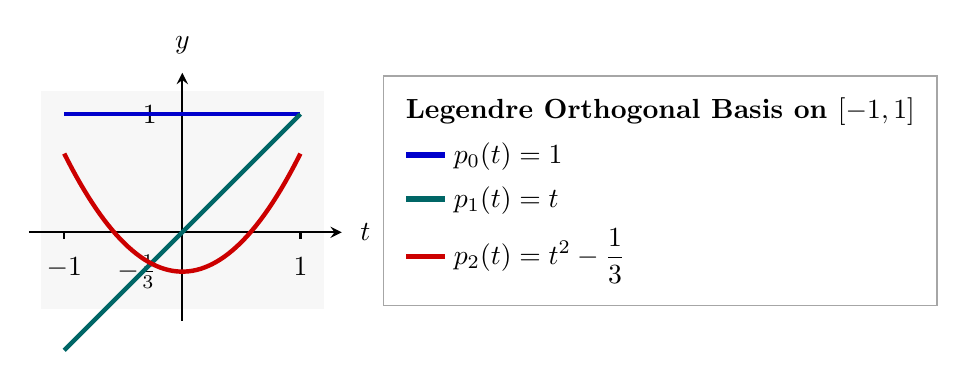
\begin{tikzpicture}[scale=1.5]
    % Layer 1: Background plot window
    \fill[gray!6] (-1.2,-0.65) rectangle (1.2,1.2);
    % Layer 2: Coordinate axes and explicit tick marks
    \draw[->, >=stealth, thick, black] (-1.3,0) -- (1.35,0) node[right=3pt, black] {$t$};
    \draw[->, >=stealth, thick, black] (0,-0.75) -- (0,1.35) node[above=3pt, black] {$y$};
    \draw[thick] (-1,0) -- (-1,-0.06) node[below=3pt, black] {$-1$};
    \draw[thick] (1,0) -- (1,-0.06) node[below=3pt, black] {$1$};
    \draw[thick] (0,1) -- (-0.06,1) node[left=3pt, black] {$1$};
    \draw[thick] (0,-0.333) -- (-0.06,-0.333) node[left=3pt, black] {$-\frac{1}{3}$};
    % Layer 3: Orthogonal Legendre polynomials
    \draw[ultra thick, blue!80!black, domain=-1:1, samples=2] plot (\x, {1});
    \draw[ultra thick, teal!80!black, domain=-1:1, samples=2] plot (\x, {\x});
    \draw[ultra thick, red!80!black, domain=-1:1, samples=60] plot (\x, {\x*\x - 0.3333});
    % Layer 4: Single-node anchored legend
    \node[align=left, inner sep=8pt, draw=black!35, fill=white, anchor=west, text=black] at (1.7, 0.35) {
        \textbf{Legendre Orthogonal Basis on $[-1, 1]$}\\[4pt]
        {\color{blue!80!black}\rule[2pt]{14pt}{2pt}} $\displaystyle p_0(t) = 1$\\[4pt]
        {\color{teal!80!black}\rule[2pt]{14pt}{2pt}} $\displaystyle p_1(t) = t$\\[4pt]
        {\color{red!80!black}\rule[2pt]{14pt}{2pt}} $\displaystyle p_2(t) = t^2 - \frac{1}{3}$
    };
\end{tikzpicture}
\caption{The first three orthogonal Legendre polynomials in $C[-1, 1]$ obtained in Exercise 31.}
\end{figure}

\textbf{Exercise 32 (Original Problem):} Let $V$ be the space $C[-2, 2]$ with the inner product of Example 7. Find an orthogonal basis for the subspace spanned by the polynomials $1, t$, and $t^2$.

\textbf{Solution:}
Apply Gram--Schmidt with $\langle f, g \rangle = \int_{-2}^2 f(t)g(t)\,dt$:
\begin{enumerate}
    \item Set $p_0(t) = 1$. Then $\langle p_0, p_0 \rangle = \int_{-2}^2 1\,dt = 4$.
    \item Compute $\langle t, p_0 \rangle = \int_{-2}^2 t\,dt = 0$ (odd function on $[-2, 2]$). Thus $p_1(t) = t$.
    \item For $p_2$, compute:
    \begin{align*}
        \langle t^2, p_0 \rangle &= \int_{-2}^2 t^2\,dt = \left[\frac{t^3}{3}\right]_{-2}^2 = \frac{8}{3} - \left(-\frac{8}{3}\right) = \frac{16}{3}, \\
        \langle t^2, p_1 \rangle &= \int_{-2}^2 t^3\,dt = 0 \quad \text{(odd integrand on } [-2, 2]\text{)}.
    \end{align*}
    Therefore,
    \[
        p_2(t) = t^2 - \frac{16/3}{4}(1) - 0 = t^2 - \frac{4}{3}.
    \]
\end{enumerate}
\textbf{Final Answer:} An orthogonal basis is $\displaystyle \left\{1,\; t,\; t^2 - \frac{4}{3}\right\}$.

\textbf{Exercise 33 (T) (Original Problem):} Let $\mathbb{P}_4$ have the inner product as in Example 5, and let $p_0, p_1, p_2$ be the orthogonal polynomials from that example. Using your matrix program, apply the Gram--Schmidt process to the set $\{p_0, p_1, p_2, t^3, t^4\}$ to create an orthogonal basis for $\mathbb{P}_4$.

\textbf{Solution:}
In Example 5, the inner product on $\mathbb{P}_4$ is evaluation at $-2, -1, 0, 1, 2$, and we are given $p_0(t) = 1$, $p_1(t) = t$, $p_2(t) = t^2 - 2$. Under the evaluation isomorphism onto $\mathbb{R}^5$, their value vectors and squared norms are:
\[
    p_0 \leftrightarrow \begin{bmatrix} 1 \\ 1 \\ 1 \\ 1 \\ 1 \end{bmatrix},\; \|p_0\|^2 = 5, \qquad
    p_1 \leftrightarrow \begin{bmatrix} -2 \\ -1 \\ 0 \\ 1 \\ 2 \end{bmatrix},\; \|p_1\|^2 = 10, \qquad
    p_2 \leftrightarrow \begin{bmatrix} 2 \\ -1 \\ -2 \\ -1 \\ 2 \end{bmatrix},\; \|p_2\|^2 = 14.
\]
\textbf{Step 1 (Construct $p_3$ from $t^3$):} From Exercise 11, $t^3 \leftrightarrow (-8, -1, 0, 1, 8)^T$, and
\[
    \langle t^3, p_0 \rangle = 0, \qquad \langle t^3, p_1 \rangle = 34, \qquad \langle t^3, p_2 \rangle = 0.
\]
Hence,
\[
    p_3(t) = t^3 - \frac{34}{10}p_1(t) = t^3 - \frac{17}{5}t.
\]
Its vector of values at $(-2, -1, 0, 1, 2)$ is $\left(-\frac{6}{5},\; \frac{12}{5},\; 0,\; -\frac{12}{5},\; \frac{6}{5}\right)^T = \frac{6}{5}(-1, 2, 0, -2, 1)^T$, with squared norm
\[
    \langle p_3, p_3 \rangle = \frac{36}{25}\bigl((-1)^2 + 2^2 + 0^2 + (-2)^2 + 1^2\bigr) = \frac{36}{25}(10) = \frac{72}{5}.
\]
\textbf{Step 2 (Construct $p_4$ from $t^4$):} The value vector of $t^4$ at $(-2, -1, 0, 1, 2)$ is $(16, 1, 0, 1, 16)^T$. Compute its inner products with $p_0, p_1, p_2, p_3$:
\begin{align*}
    \langle t^4, p_0 \rangle &= 16 + 1 + 0 + 1 + 16 = 34, \\
    \langle t^4, p_1 \rangle &= 16(-2) + 1(-1) + 0 + 1(1) + 16(2) = 0, \\
    \langle t^4, p_2 \rangle &= 16(2) + 1(-1) + 0(-2) + 1(-1) + 16(2) = 62, \\
    \langle t^4, p_3 \rangle &= \frac{6}{5}\bigl(16(-1) + 1(2) + 0(0) + 1(-2) + 16(1)\bigr) = 0.
\end{align*}
Therefore,
\begin{align*}
    p_4(t) &= t^4 - \frac{34}{5}p_0(t) - \frac{62}{14}p_2(t) \\
    &= t^4 - \frac{34}{5}(1) - \frac{31}{7}(t^2 - 2) \\
    &= t^4 - \frac{31}{7}t^2 + \frac{62}{7} - \frac{34}{5} \\
    &= t^4 - \frac{31}{7}t^2 + \frac{310 - 238}{35} = t^4 - \frac{31}{7}t^2 + \frac{72}{35}.
\end{align*}
(As a check, the value vector of $p_4$ at $(-2,-1,0,1,2)$ is $\frac{12}{35}(1, -4, 6, -4, 1)^T$, which is orthogonal to the value vectors of $p_0, p_1, p_2, p_3$.)\\
\textbf{Final Answer:} An orthogonal basis for $\mathbb{P}_4$ is
\[
    \left\{1,\; t,\; t^2 - 2,\; t^3 - \frac{17}{5}t,\; t^4 - \frac{31}{7}t^2 + \frac{72}{35}\right\}.
\]
(Equivalently, with integer value vectors, $\left\{1,\; t,\; t^2 - 2,\; \frac{5}{6}t^3 - \frac{17}{6}t,\; \frac{35}{12}t^4 - \frac{155}{12}t^2 + 6\right\}$.)

\textbf{Exercise 34 (T) (Original Problem):} Let $V$ be the space $C[0, 2\pi]$ with the inner product of Example 7. Use the Gram--Schmidt process to create an orthogonal basis for the subspace spanned by $\{1, \cos t, \cos^2 t, \cos^3 t\}$. Use a matrix program or computational program to compute the appropriate definite integrals.

\textbf{Solution:}
Let $\langle f, g \rangle = \int_0^{2\pi} f(t)g(t)\,dt$. We first tabulate the exact integrals $\int_0^{2\pi} \cos^k t\,dt$:
\begin{itemize}
    \item For every odd integer $k$, $\cos^k(t + \pi) = -\cos^k t$, so over a full $2\pi$ period $\int_0^{2\pi} \cos^k t\,dt = 0$.
    \item For $k = 0$: $\int_0^{2\pi} 1\,dt = 2\pi$.
    \item For $k = 2$: $\int_0^{2\pi} \cos^2 t\,dt = \int_0^{2\pi} \frac{1 + \cos 2t}{2}\,dt = \pi$.
    \item For $k = 4$:
    \[
        \int_0^{2\pi} \cos^4 t\,dt = \int_0^{2\pi} \left(\frac{1 + \cos 2t}{2}\right)^2 dt = \frac{1}{4}\int_0^{2\pi} \left(1 + 2\cos 2t + \frac{1 + \cos 4t}{2}\right) dt = \frac{1}{4}\left(2\pi + 0 + \pi\right) = \frac{3\pi}{4}.
    \]
\end{itemize}
Now apply Gram--Schmidt to $f_0(t) = 1$, $f_1(t) = \cos t$, $f_2(t) = \cos^2 t$, $f_3(t) = \cos^3 t$:
\begin{enumerate}
    \item Set $q_0(t) = 1$, with $\langle q_0, q_0 \rangle = 2\pi$.
    \item Compute $\langle f_1, q_0 \rangle = \int_0^{2\pi} \cos t\,dt = 0$. Thus $q_1(t) = \cos t$, with $\langle q_1, q_1 \rangle = \pi$.
    \item For $q_2$, compute:
    \[
        \langle f_2, q_0 \rangle = \int_0^{2\pi} \cos^2 t\,dt = \pi, \qquad \langle f_2, q_1 \rangle = \int_0^{2\pi} \cos^3 t\,dt = 0.
    \]
    Hence,
    \[
        q_2(t) = \cos^2 t - \frac{\pi}{2\pi}(1) = \cos^2 t - \frac{1}{2} = \frac{1}{2}\cos 2t.
    \]
    Note that $\langle q_2, q_2 \rangle = \int_0^{2\pi} \frac{1}{4}\cos^2(2t)\,dt = \frac{\pi}{4}$.
    \item For $q_3$, compute:
    \begin{align*}
        \langle f_3, q_0 \rangle &= \int_0^{2\pi} \cos^3 t\,dt = 0, \\
        \langle f_3, q_1 \rangle &= \int_0^{2\pi} \cos^4 t\,dt = \frac{3\pi}{4}, \\
        \langle f_3, q_2 \rangle &= \int_0^{2\pi} \cos^3 t \left(\cos^2 t - \frac{1}{2}\right) dt = \int_0^{2\pi} \cos^5 t\,dt - \frac{1}{2}\int_0^{2\pi} \cos^3 t\,dt = 0.
    \end{align*}
    Hence,
    \[
        q_3(t) = \cos^3 t - \frac{3\pi/4}{\pi}\cos t = \cos^3 t - \frac{3}{4}\cos t = \frac{1}{4}\cos 3t.
    \]
\end{enumerate}
\textbf{Final Answer:} An orthogonal basis is
\[
    \left\{1,\; \cos t,\; \cos^2 t - \frac{1}{2},\; \cos^3 t - \frac{3}{4}\cos t\right\} = \left\{1,\; \cos t,\; \frac{1}{2}\cos 2t,\; \frac{1}{4}\cos 3t\right\}.
\]

\newpage
\section{In-Depth Analysis of Problems and Techniques}

\subsection{Problem Types and General Approach}

\begin{description}
    \item[Type 1: Direct Computation of Inner Products, Norms, and Orthogonality (Exercises 1, 3--6, 27--30)] \leavevmode \\
    \emph{Strategic Workflow:} Identify the explicit formula for $\langle \mathbf{u}, \mathbf{v} \rangle$ (weighted sum in $\mathbb{R}^n$, evaluation sum in $\mathbb{P}_n$, or definite integral in $C[a, b]$). Substitute the vectors/functions directly, compute $\langle \mathbf{u}, \mathbf{v} \rangle$ for orthogonality or angles, compute $\langle \mathbf{v}, \mathbf{v} \rangle$ for $\|\mathbf{v}\|^2$, and take the nonnegative square root at the very end to obtain $\|\mathbf{v}\|$. For orthogonality conditions (Exercise 1b), set $\langle \mathbf{z}, \mathbf{y} \rangle = 0$ and solve the resulting homogeneous linear equation.

    \item[Type 2: Orthogonal Projections and Best Approximation (Exercises 7--8, 10--11)] \leavevmode \\
    \emph{Strategic Workflow:} Confirm that the spanning set $\{\mathbf{w}_1, \dots, \mathbf{w}_p\}$ of the target subspace $W$ is already orthogonal. If so, evaluate each projection coefficient $c_i = \langle \mathbf{v}, \mathbf{w}_i \rangle / \langle \mathbf{w}_i, \mathbf{w}_i \rangle$ and form $\operatorname{proj}_W \mathbf{v} = \sum_{i=1}^p c_i \mathbf{w}_i$. By the Best Approximation Theorem, this projection is automatically the unique closest vector in $W$ to $\mathbf{v}$.

    \item[Type 3: Gram--Schmidt Orthogonalization and Basis Rescaling (Exercises 9, 12, 31--34)] \leavevmode \\
    \emph{Strategic Workflow:} Build the orthogonal basis sequentially. At step $k$, project the new vector $\mathbf{x}_k$ onto the previously constructed orthogonal vectors $\{\mathbf{v}_1, \dots, \mathbf{v}_{k-1}\}$ and subtract that projection from $\mathbf{x}_k$. If the problem specifies target evaluation values (Exercises 9b, 12), evaluate the raw orthogonal polynomial at the nodes and multiply by the reciprocal scalar factor to match the prescribed vector of values.

    \item[Type 4: Verification of Inner Product Axioms for Pullback Constructions (Exercises 13--14)] \leavevmode \\
    \emph{Strategic Workflow:} Systematically verify Axioms 1--4. Axioms 1--3 almost always follow immediately from linearity of the map ($A$ or $T$) and the properties of the target dot product. Axiom 4 is the critical step: express $\langle \mathbf{u}, \mathbf{u} \rangle = \|T(\mathbf{u})\|_2^2 \ge 0$, then invoke \emph{invertibility} of $A$ (Exercise 13) or \emph{injectivity} of $T$ (Exercise 14) to prove that $T(\mathbf{u}) = \mathbf{0}$ forces $\mathbf{u} = \mathbf{0}$.

    \item[Type 5: Axiomatic Proofs and Abstract Vector Identities (Practice Problems 1--2, Exercises 15--24)] \leavevmode \\
    \emph{Strategic Workflow:} Treat $\langle \cdot, \cdot \rangle$ strictly as an abstract bilinear symmetric positive-definite form—never assume coordinates or integrals. Use Axiom 1 (symmetry) to move operations from the second slot to the first slot (Exercises 15, 21), expand squared norms as $\langle \mathbf{u} \pm \mathbf{v}, \mathbf{u} \pm \mathbf{v} \rangle$ (Exercises 16--18), and test True/False claims against Axiom 4, bilinearity, and Cauchy--Schwarz (Exercises 19--24).

    \item[Type 6: Inequality Proofs via Cauchy--Schwarz (Exercises 2, 25--26)] \leavevmode \\
    \emph{Strategic Workflow:} Either verify $|\langle \mathbf{x}, \mathbf{y} \rangle|^2 \le \|\mathbf{x}\|^2 \|\mathbf{y}\|^2$ numerically for given vectors (Exercise 2) or select strategic vectors $\mathbf{u}, \mathbf{v} \in \mathbb{R}^2$ whose dot product produces the desired cross-term ($2\sqrt{ab}$ or $a+b$) while their squared norms yield the bounding quadratic/sum expressions ($a+b$ or $a^2+b^2$).
\end{description}

\subsection{Key Algebraic and Calculus Manipulations}

\begin{enumerate}
    \item \textbf{The Evaluation Isomorphism ($\mathbb{P}_n \cong \mathbb{R}^{n+1}$):} In Exercises 3--12 and 33, rather than multiplying polynomials symbolically at every step, converting each polynomial $p$ into its vector of values $(p(t_0), \dots, p(t_n))^T \in \mathbb{R}^{n+1}$ reduces inner products and projections to ordinary dot products in $\mathbb{R}^{n+1}$. Only after finding the projection coefficients do we assemble the polynomial in $t$.
    \item \textbf{Parity Symmetry on Symmetric Nodes and Intervals:} In Exercises 9--12, 31--33, and 34, evaluating an odd function against an even function over symmetric nodes (e.g., $\{-3, -1, 1, 3\}$ or $\{-2, -1, 0, 1, 2\}$) or a symmetric interval ($[-1, 1]$, $[-2, 2]$, or a full period $[0, 2\pi]$ for odd powers of $\cos t$) immediately gives $0$, eliminating half of the Gram--Schmidt projection integrals before any arithmetic is performed.
    \item \textbf{Bilinear Expansion of Squared Norms:} In Exercises 16--18, writing $\|\mathbf{u} \pm \mathbf{v}\|^2 = \langle \mathbf{u} \pm \mathbf{v}, \mathbf{u} \pm \mathbf{v} \rangle = \|\mathbf{u}\|^2 \pm 2\langle \mathbf{u}, \mathbf{v} \rangle + \|\mathbf{v}\|^2$ systematically unlocks both the Polarization Identity (Exercise 17, by subtraction) and the Parallelogram Law (Exercise 18, by addition).
    \item \textbf{Scalar Scaling to Match Boundary/Node Conditions:} In Exercises 9b and 12, Gram--Schmidt produced $t^2 - 5$ and $t^3 - \frac{17}{5}t$, whose values at the nodes were multiples of the requested vectors. Because any nonzero scalar multiple of an orthogonal vector remains orthogonal to the preceding basis vectors, multiplying by $\frac{1}{4}$ or $\frac{5}{6}$ adjusts the scale without breaking orthogonality.
    \item \textbf{Trigonometric Power-Reduction and Triple-Angle Identities:} In Exercise 34, evaluating $\int_0^{2\pi} \cos^4 t\,dt$ required replacing $\cos^2 t$ by $\frac{1+\cos 2t}{2}$ twice, while recognizing $\cos^3 t - \frac{3}{4}\cos t = \frac{1}{4}\cos 3t$ revealed that Gram--Schmidt on $\{1, \cos t, \cos^2 t, \cos^3 t\}$ reconstructs the Fourier cosine basis.
    \item \textbf{Square-Root Vector Embedding:} In Exercise 25, choosing $\mathbf{u} = (\sqrt{a}, \sqrt{b})^T$ and $\mathbf{v} = (\sqrt{b}, \sqrt{a})^T$ was crucial because the squared norms $\|\mathbf{u}\|^2 = \|\mathbf{v}\|^2 = a+b$ naturally remove the radicals on the right-hand side of Cauchy--Schwarz while keeping $\sqrt{ab}$ on the left.
\end{enumerate}

\newpage
\section{Cheatsheet and Tips for Success}

\subsection{Essential Formula Summary}

\renewcommand{\arraystretch}{1.5}
\begin{tabularx}{\textwidth}{>{\raggedright\arraybackslash}p{4.4cm} >{$\displaystyle}l<{$} X}
\toprule
\textbf{Tool} & \textbf{Expression} & \textbf{Quick Note} \\
\midrule
Bilinearity in Slot 2 & \langle \mathbf{u}, a\mathbf{v} + b\mathbf{w} \rangle = a\langle \mathbf{u}, \mathbf{v} \rangle + b\langle \mathbf{u}, \mathbf{w} \rangle & Derived from Axioms 1--3; inner products are linear in both slots. \\
\addlinespace[4pt]
Scaling Both Slots & \langle c\mathbf{u}, c\mathbf{v} \rangle = c^2 \langle \mathbf{u}, \mathbf{v} \rangle & Norm satisfies $\|c\mathbf{u}\| = |c|\,\|\mathbf{u}\|$. \\
\addlinespace[4pt]
Gram--Schmidt Step & \mathbf{v}_k = \mathbf{x}_k - \sum_{j=1}^{k-1} \frac{\langle \mathbf{x}_k, \mathbf{v}_j \rangle}{\langle \mathbf{v}_j, \mathbf{v}_j \rangle}\mathbf{v}_j & Only valid once $\{\mathbf{v}_1, \dots, \mathbf{v}_{k-1}\}$ are already orthogonal. \\
\addlinespace[4pt]
Polarization Identity & \langle \mathbf{u}, \mathbf{v} \rangle = \frac{1}{4}\left(\|\mathbf{u}+\mathbf{v}\|^2 - \|\mathbf{u}-\mathbf{v}\|^2\right) & Recovers the inner product purely from norms. \\
\addlinespace[4pt]
Parallelogram Law & \|\mathbf{u}+\mathbf{v}\|^2 + \|\mathbf{u}-\mathbf{v}\|^2 = 2\|\mathbf{u}\|^2 + 2\|\mathbf{v}\|^2 & Necessary and sufficient condition for a norm to come from an inner product. \\
\bottomrule
\end{tabularx}

\subsection{Speed Tricks and Shortcuts}

\begin{itemize}
    \item \textbf{Check Parity First:} Before computing any integral on $[-a, a]$ or discrete sum on symmetric nodes $\{-b, -a, a, b\}$, separate polynomials into even and odd parts. Any inner product between an even function and an odd function is automatically $0$.
    \item \textbf{Use Column Vectors for Evaluation Inner Products:} Write the node evaluations of every basis polynomial in a table or column vectors first; all projections reduce to integer dot products.
    \item \textbf{Keep Rational Denominators Factored Until the End:} In Gram--Schmidt, you may temporarily clear denominators when computing $\mathbf{v}_k$ (since any nonzero scalar multiple $\tilde{\mathbf{v}}_k = \lambda \mathbf{v}_k$ gives the exact same projection $\frac{\langle \mathbf{x}, \tilde{\mathbf{v}}_k \rangle}{\langle \tilde{\mathbf{v}}_k, \tilde{\mathbf{v}}_k \rangle}\tilde{\mathbf{v}}_k$), drastically reducing fraction arithmetic.
    \item \textbf{Squared-Norm Check for Cauchy--Schwarz:} To verify $|\langle \mathbf{u}, \mathbf{v} \rangle| \le \|\mathbf{u}\|\,\|\mathbf{v}\|$ without ugly radicals, verify $|\langle \mathbf{u}, \mathbf{v} \rangle|^2 \le \|\mathbf{u}\|^2 \|\mathbf{v}\|^2$ instead (since both sides are nonnegative).
\end{itemize}

\subsection{Common Pitfalls and Traps}

\begin{itemize}
    \item \textbf{Forgetting the Denominator Square:} Writing $\frac{\langle \mathbf{v}, \mathbf{w} \rangle}{\|\mathbf{w}\|}\mathbf{w}$ instead of $\frac{\langle \mathbf{v}, \mathbf{w} \rangle}{\langle \mathbf{w}, \mathbf{w} \rangle}\mathbf{w} = \frac{\langle \mathbf{v}, \mathbf{w} \rangle}{\|\mathbf{w}\|^2}\mathbf{w}$ is the single most common error in projections unless $\mathbf{w}$ is already a unit vector.
    \item \textbf{Linearity Trap with Equal Scalars:} Writing $\langle c\mathbf{u}, c\mathbf{v} \rangle = c\langle \mathbf{u}, \mathbf{v} \rangle$ (Exercise 22) misses the second factor of $c$; the true identity is $c^2 \langle \mathbf{u}, \mathbf{v} \rangle$.
    \item \textbf{Zero-Product Fallacy:} Assuming $\langle \mathbf{u}, \mathbf{v} \rangle = 0$ implies $\mathbf{u} = \mathbf{0}$ or $\mathbf{v} = \mathbf{0}$ (Exercise 20). Orthogonality of nonzero vectors is the entire point of inner product spaces!
    \item \textbf{Ignoring Injectivity in Axiom 4:} Defining $\langle \mathbf{u}, \mathbf{v} \rangle = (A\mathbf{u})\cdot(A\mathbf{v})$ for a \emph{non-invertible} matrix $A$ fails Axiom 4 because any nonzero $\mathbf{u} \in \operatorname{Nul} A$ satisfies $\langle \mathbf{u}, \mathbf{u} \rangle = 0$.
    \item \textbf{Insufficient Evaluation Nodes:} An evaluation inner product on $\mathbb{P}_n$ requires at least $n+1$ distinct points. Using only $3$ nodes on $\mathbb{P}_3$ fails Axiom 4 because a nonzero cubic can vanish at $3$ points (e.g., $p(t) = (t+1)t(t-1)$).
\end{itemize}

\subsection{Problem Recognition Guide}

\begin{itemize}
    \item \textbf{``Show that $\langle \cdot, \cdot \rangle$ defines an inner product...''} $\longrightarrow$ Check Axioms 1--4 systematically; isolate what guarantees $\langle \mathbf{u}, \mathbf{u} \rangle = 0 \implies \mathbf{u} = \mathbf{0}$ (positive weights, $n+1$ nodes for $\mathbb{P}_n$, continuity of $f^2$, or injectivity of $T$).
    \item \textbf{``Find the best approximation to $f$ by functions in $W$...''} $\longrightarrow$ Compute $\operatorname{proj}_W f$ using an orthogonal basis of $W$ (if the given basis is not orthogonal, run Gram--Schmidt first!).
    \item \textbf{``Show inequality involving $a, b$ using Cauchy--Schwarz...''} $\longrightarrow$ Reverse-engineer $\mathbf{u}, \mathbf{v} \in \mathbb{R}^2$ so $\mathbf{u} \cdot \mathbf{v}$ matches the left-hand side and $\|\mathbf{u}\| \|\mathbf{v}\|$ matches the right-hand side.
\end{itemize}

\newpage
\section{Conceptual Synthesis and the Big Picture}

\subsection{Thematic Connections}

The central theme of Section 6.7 is **geometric abstraction via structural axioms**: identifying the minimal algebraic rules (Axioms 1--4) that make Euclidean length, orthogonality, and least-squares projection work, and transferring that entire geometric engine to spaces of polynomials, signals, and continuous functions.

This theme mirrors two foundational ideas across mathematics:
\begin{enumerate}
    \item \textbf{Algebraic Axiomatization:} Just as vector spaces abstracted $\mathbb{R}^n$ linear combinations by extracting eight vector-space axioms (Chapter 4), inner product spaces abstract the dot product by extracting four inner-product axioms. Any theorem proved purely from those four axioms (Cauchy--Schwarz, Triangle Inequality, Pythagorean Theorem, Best Approximation) immediately holds in every inner product space simultaneously.
    \item \textbf{Approximation as Orthogonal Projection:} In calculus, Taylor polynomials approximate a function $f$ locally around a single point $t_0$ using derivatives. In an inner product space, orthogonal projection approximates $f$ \emph{globally} across an interval $[a, b]$ (via $C[a, b]$) or across a sampling grid (via evaluation nodes) by minimizing the global mean-square error $\|f - g\|^2$.
\end{enumerate}

\subsection{Forward and Backward Links}

\subsubsection*{Backward Links (Where Section 6.7 Comes From)}
Section 6.7 is the direct generalization of Sections 6.1--6.6:
\begin{itemize}
    \item Theorem 1 of Section 6.1 listed the four algebraic properties of the standard dot product in $\mathbb{R}^n$; Section 6.7 turns those four conclusions into the defining axioms of an inner product.
    \item Orthogonal bases, the Gram--Schmidt process (Section 6.4), and least-squares best approximation (Sections 6.3 and 6.5) were originally restricted to $\mathbb{R}^n$. Section 6.7 reveals that none of those theorems truly depended on $\mathbb{R}^n$ coordinates—they depended only on the inner product structure.
    \item Definite integration and Riemann sums from single-variable calculus provide the limiting bridge from discrete data-point sums to continuous $L^2$-type inner products on $C[a, b]$.
\end{itemize}

\subsubsection*{Forward Links (Where Section 6.7 Leads)}
The concepts of Section 6.7 form the indispensable bedrock for advanced pure and applied mathematics:
\begin{itemize}
    \item \textbf{Weighted Least-Squares and Fourier Series (Section 6.8):} Immediately following this section, weighted inner products on $\mathbb{R}^n$ model heteroscedastic statistical regression (weighting reliable data points more heavily), while the integral inner product on $C[0, 2\pi]$ yields trigonometric Fourier series approximations.
    \item \textbf{Differential Equations and Sturm--Liouville Theory:} Solving boundary-value PDEs (heat, wave, and Schr\"{o}dinger equations) by separation of variables produces eigenfunctions (Legendre, Bessel, Hermite, and Chebyshev polynomials) that are mutually orthogonal under weighted integral inner products.
    \item \textbf{Functional Analysis and Hilbert Spaces:} Completing an inner product space with respect to the metric $d(\mathbf{u}, \mathbf{v}) = \|\mathbf{u} - \mathbf{v}\|$ produces a \emph{Hilbert space} (such as $L^2([a, b])$), the mathematical setting of quantum mechanics, signal processing, and Sobolev spaces for weak solutions of PDEs.
\end{itemize}

\newpage
\section{Abstract Real-World Modeling in AI, ML, and Quantitative Finance}

\subsection{Concrete Scenarios}

\begin{enumerate}
    \item \textbf{Reproducing Kernel Hilbert Spaces (RKHS) and Support Vector Machines in Machine Learning:}
    In nonlinear classification and Kernel Ridge Regression, raw inputs $\mathbf{x} \in \mathbb{R}^d$ are mapped via a feature map $\Phi: \mathbb{R}^d \to \mathcal{H}$ into a possibly infinite-dimensional inner product space (an RKHS $\mathcal{H}$). Algorithms never need to compute $\Phi(\mathbf{x})$ explicitly; instead, by the ``kernel trick,'' every distance, projection, and hyperplane margin is computed solely through the inner product $k(\mathbf{x}, \mathbf{x}') = \langle \Phi(\mathbf{x}), \Phi(\mathbf{x}') \rangle_{\mathcal{H}}$. Positive-definiteness (Axiom 4) of the inner product corresponds directly to Mercer's condition on the kernel matrix, guaranteeing convex optimization with a unique global minimum.

    \item \textbf{Mean-Variance Hedging and Conditional Expectation in Quantitative Finance:}
    In an incomplete financial market modeled on a probability space $(\Omega, \mathcal{F}, \mathbb{P})$, square-integrable random payoffs form the inner product space $L^2(\Omega, \mathcal{F}, \mathbb{P})$ with $\langle X, Y \rangle = \mathbb{E}[XY]$. A derivative contract with payoff $H \in L^2$ cannot generally be replicated exactly using traded assets. By the Best Approximation Theorem in $L^2$, the optimal self-financing hedging strategy minimizes the quadratic hedging error $\mathbb{E}[(H - g)^2] = \|H - g\|_{L^2}^2$ over the subspace $\mathcal{G}$ of attainable terminal payoffs—meaning the optimal hedge is literally the orthogonal projection $\operatorname{proj}_{\mathcal{G}} H$. Moreover, conditional expectation $\mathbb{E}[H \mid \mathcal{F}_t]$ is itself the orthogonal projection of $H$ onto the subspace $L^2(\Omega, \mathcal{F}_t, \mathbb{P})$.

    \item \textbf{Scaled Dot-Product Attention and Metric Learning in Generative AI:}
    In Transformer architectures, attention weights between a query $\mathbf{q} \in \mathbb{R}^{d_k}$ and a key $\mathbf{k} \in \mathbb{R}^{d_k}$ are computed via scaled inner products $\frac{\langle \mathbf{q}, \mathbf{k} \rangle}{\sqrt{d_k}}$. When learned projection matrices $W_Q, W_K$ map token embeddings into a shared latent space, the attention similarity $\langle W_Q \mathbf{x}, W_K \mathbf{y} \rangle$ generalizes to Mahalanobis-type pullback inner products $\langle \mathbf{u}, \mathbf{v} \rangle_A = (A\mathbf{u})^T(A\mathbf{v})$ (precisely Exercise 13) when $W_Q = W_K = A$ is invertible, learning an anisotropic geometry tailored to semantic similarity.
\end{enumerate}

\subsection{Model Problem Setup: $L^2$-Optimal Quadratic Hedging of Contingent Claims}

We formalize Scenario 2 (Mean-Variance / Quadratic Hedging in an Incomplete Market) as a rigorous mathematical optimization problem in an inner product space.

\subsubsection*{1. State Space, Filtration, and Inner Product Structure}
Let $(\Omega, \mathcal{F}, \{\mathcal{F}_t\}_{t \in [0, T]}, \mathbb{P})$ be a complete filtered probability space over a finite trading horizon $[0, T]$, satisfying the usual conditions. Consider the real inner product space of square-integrable terminal payoffs:
\[
    V = L^2(\Omega, \mathcal{F}_T, \mathbb{P}), \qquad \langle X, Y \rangle_{L^2} := \mathbb{E}[XY], \qquad \|X\|_{L^2} := \sqrt{\mathbb{E}[X^2]}.
\]
(Note that elements of $L^2$ are equivalence classes of random variables agreeing $\mathbb{P}$-almost surely, ensuring Axiom 4 holds: $\mathbb{E}[X^2] = 0 \implies X = 0$ $\mathbb{P}$-a.s.)

\subsubsection*{2. Market Dynamics and Admissible Payoff Subspace}
Suppose a discounted risky asset $S = (S_t)_{t \in [0, T]}$ follows a semimartingale stochastic differential equation driven by a standard Brownian motion $W_t$ and a stochastic volatility factor $v_t$ (introducing market incompleteness via an unspanned Brownian motion $B_t$):
\begin{align*}
    dS_t &= \mu_t S_t\,dt + \sqrt{v_t} S_t\,dW_t, \\
    dv_t &= \kappa(\bar{v} - v_t)\,dt + \xi \sqrt{v_t}\left(\rho\,dW_t + \sqrt{1 - \rho^2}\,dB_t\right),
\end{align*}
where $\kappa, \bar{v}, \xi > 0$, $|\rho| < 1$, and $W_t \perp B_t$. By It\^{o}'s Lemma, any smooth function $f(t, S_t, v_t)$ evolves according to both $dW_t$ and $dB_t$, whereas trading only in $S_t$ and a risk-free num\'{e}raire yields terminal wealth
\[
    G_T(c, \theta) = c + \int_0^T \theta_t\,dS_t,
\]
where $c \in \mathbb{R}$ is initial capital and $\theta = (\theta_t)_{t \in [0, T]}$ belongs to the set $\Theta$ of predictable strategies satisfying $\mathbb{E}\left[\int_0^T \theta_t^2\,d\langle S \rangle_t + \left(\int_0^T |\theta_t \mu_t S_t|\,dt\right)^2\right] < \infty$. Let
\[
    \mathcal{G} := \left\{ c + \int_0^T \theta_t\,dS_t : c \in \mathbb{R},\; \theta \in \Theta \right\} \subset L^2(\Omega, \mathcal{F}_T, \mathbb{P})
\]
denote the linear subspace of $L^2$-attainable terminal payoffs.

\subsubsection*{3. Variational Formulation and Orthogonal Projection Optimality}
Given an $\mathcal{F}_T$-measurable contingent claim $H \in L^2(\Omega, \mathcal{F}_T, \mathbb{P})$ (e.g., a European option $H = (S_T - K)^+$), the quadratic hedging problem seeks the initial capital $c^*$ and dynamic trading strategy $\theta^* \in \Theta$ minimizing expected squared replication error:
\[
    \min_{(c, \theta) \in \mathbb{R} \times \Theta} \mathcal{L}(c, \theta), \qquad \text{where } \mathcal{L}(c, \theta) := \mathbb{E}\!\left[\left(H - c - \int_0^T \theta_t\,dS_t\right)^2\right] = \|H - G_T(c, \theta)\|_{L^2}^2.
\]
Under the assumption that $\mathcal{G}$ is a closed subspace of $L^2(\Omega, \mathcal{F}_T, \mathbb{P})$ (guaranteed under standard bounded mean-variance tradeoff conditions), the Best Approximation Theorem implies that a unique optimal attainable payoff $G_T^* = \operatorname{proj}_{\mathcal{G}} H$ exists and is uniquely characterized by the **orthogonality condition**:
\[
    \langle H - G_T^*, \, g \rangle_{L^2} = \mathbb{E}\!\left[\left(H - c^* - \int_0^T \theta_t^*\,dS_t\right) g\right] = 0 \qquad \forall g \in \mathcal{G}.
\]
In particular, testing against $g = 1 \in \mathcal{G}$ forces the hedging error to have zero mean ($\mathbb{E}[H - G_T^*] = 0$), and testing against elementary stochastic integrals characterizes the F\"{o}llmer--Sondermann optimal hedging strategy $\theta^*$, decomposing the claim orthogonally into $H = G_T^* + \varepsilon_{\perp}$ with $\mathbb{E}[G_T^* \varepsilon_{\perp}] = 0$ and minimal residual risk $\|\varepsilon_{\perp}\|_{L^2}^2 = \|H\|_{L^2}^2 - \|G_T^*\|_{L^2}^2$.

\newpage
\section{Common Variations and Untested Concepts}

While Section 6.7 covers real inner products, discrete evaluations, and unweighted $C[a, b]$ integrals, a complete mastery of inner product spaces requires understanding four standard extensions not tested in the homework set.

\subsection{Variation 1: Complex Inner Product Spaces (Hermitian Forms)}
Over the complex field $\mathbb{C}$, defining $\langle \mathbf{u}, \mathbf{v} \rangle = \sum u_j v_j$ fails Axiom 4 because $(i)^2 = -1 < 0$. To guarantee $\langle \mathbf{u}, \mathbf{u} \rangle \ge 0$, Axiom 1 is replaced by **conjugate symmetry**: $\langle \mathbf{u}, \mathbf{v} \rangle = \overline{\langle \mathbf{v}, \mathbf{u} \rangle}$. Consequently, $\langle \mathbf{u}, c\mathbf{v} \rangle = \overline{c}\langle \mathbf{u}, \mathbf{v} \rangle$ (conjugate linearity in the second slot).

\textbf{Worked Example:} Compute $\langle \mathbf{u}, \mathbf{v} \rangle$ and $\|\mathbf{u}\|$ in $\mathbb{C}^2$ for $\mathbf{u} = (1 + i, 2)$ and $\mathbf{v} = (3 - i, i)$, where $\langle \mathbf{u}, \mathbf{v} \rangle = u_1 \overline{v_1} + u_2 \overline{v_2}$.
\begin{align*}
    \langle \mathbf{u}, \mathbf{v} \rangle &= (1 + i)\overline{(3 - i)} + (2)\overline{i} = (1 + i)(3 + i) + 2(-i) = (3 + i + 3i - 1) - 2i = 2 + 2i, \\
    \|\mathbf{u}\|^2 &= \langle \mathbf{u}, \mathbf{u} \rangle = |1 + i|^2 + |2|^2 = 2 + 4 = 6 \implies \|\mathbf{u}\| = \sqrt{6}.
\end{align*}

\subsection{Variation 2: Weighted Integral Inner Products on $C[a, b]$}
Just as $\mathbb{R}^n$ admits positive weights $w_i > 0$, $C[a, b]$ admits weighted inner products $\langle f, g \rangle_w = \int_a^b f(t)g(t)w(t)\,dt$ for any positive continuous weight function $w(t) > 0$ on $(a, b)$ (integrable at the endpoints). Important classical orthogonal polynomials—Chebyshev ($w(t) = (1-t^2)^{-1/2}$ on $(-1, 1)$), Laguerre ($w(t) = e^{-t}$ on $(0, \infty)$), and Hermite ($w(t) = e^{-t^2}$ on $(-\infty, \infty)$)—arise this way.

\textbf{Worked Example:} On $C[0, 1]$ with weight $w(t) = t$, find a polynomial of the form $p_1(t) = t - c$ orthogonal to $p_0(t) = 1$.
\[
    0 = \langle t - c, 1 \rangle_w = \int_0^1 (t - c) \cdot 1 \cdot t\,dt = \int_0^1 (t^2 - ct)\,dt = \left[\frac{t^3}{3} - \frac{c}{2}t^2\right]_0^1 = \frac{1}{3} - \frac{c}{2} \implies c = \frac{2}{3}.
\]
Thus $p_1(t) = t - \frac{2}{3}$ is orthogonal to $1$ with respect to the weight $w(t) = t$.

\subsection{Variation 3: The Frobenius Inner Product on Matrix Spaces}
On the vector space $M_{m \times n}(\mathbb{R})$ of $m \times n$ real matrices, the standard inner product is the **Frobenius inner product**:
\[
    \langle A, B \rangle_F = \operatorname{tr}(A^T B) = \sum_{i=1}^m \sum_{j=1}^n a_{ij} b_{ij}, \qquad \|A\|_F = \sqrt{\sum_{i,j} a_{ij}^2}.
\]

\textbf{Worked Example:} In $M_{2 \times 2}(\mathbb{R})$, find the orthogonal projection of $A = \begin{bmatrix} 1 & 4 \\ 0 & 3 \end{bmatrix}$ onto the subspace $W$ of symmetric matrices using the orthogonal basis $E_1 = \begin{bmatrix} 1 & 0 \\ 0 & 0 \end{bmatrix}$, $E_2 = \begin{bmatrix} 0 & 0 \\ 0 & 1 \end{bmatrix}$, $E_3 = \begin{bmatrix} 0 & 1 \\ 1 & 0 \end{bmatrix}$.
\begin{align*}
    \langle A, E_1 \rangle_F &= 1, \quad \|E_1\|_F^2 = 1; \qquad
    \langle A, E_2 \rangle_F = 3, \quad \|E_2\|_F^2 = 1; \qquad
    \langle A, E_3 \rangle_F = 4 + 0 = 4, \quad \|E_3\|_F^2 = 2.
\end{align*}
Hence $\operatorname{proj}_W A = \frac{1}{1}E_1 + \frac{3}{1}E_2 + \frac{4}{2}E_3 = \begin{bmatrix} 1 & 2 \\ 2 & 3 \end{bmatrix} = \frac{1}{2}(A + A^T)$, the symmetric part of $A$.

\subsection{Variation 4: Bessel's Inequality and Parseval's Identity}
If $\{\mathbf{e}_1, \dots, \mathbf{e}_k\}$ is any \emph{orthonormal} set in an inner product space $V$ and $\mathbf{v} \in V$, then $\operatorname{proj}_W \mathbf{v} = \sum_{j=1}^k \langle \mathbf{v}, \mathbf{e}_j \rangle \mathbf{e}_j$ has squared norm $\sum_{j=1}^k |\langle \mathbf{v}, \mathbf{e}_j \rangle|^2$. Since $\|\operatorname{proj}_W \mathbf{v}\|^2 \le \|\mathbf{v}\|^2$ by the Pythagorean Theorem, we obtain **Bessel's Inequality**:
\[
    \sum_{j=1}^k |\langle \mathbf{v}, \mathbf{e}_j \rangle|^2 \le \|\mathbf{v}\|^2,
\]
with equality (**Parseval's Identity**) if and only if $\mathbf{v} \in \operatorname{Span}\{\mathbf{e}_1, \dots, \mathbf{e}_k\}$ (or when $\{\mathbf{e}_j\}$ is a complete orthonormal system in a Hilbert space).

\textbf{Worked Example:} Verify Bessel's Inequality for $f(t) = t$ in $C[0, 1]$ using the single orthonormal function $e_1(t) = 1$ ($\|e_1\| = 1$).
\[
    |\langle f, e_1 \rangle|^2 = \left(\int_0^1 t \cdot 1\,dt\right)^2 = \left(\frac{1}{2}\right)^2 = \frac{1}{4} \le \frac{1}{3} = \int_0^1 t^2\,dt = \|f\|^2.
\]

\newpage
\section{Advanced Diagnostic Testing: Find the Flaw}

Each of the five problems below is accompanied by a complete solution that appears plausible at first glance, yet contains a **single, subtle, critical flaw**, resulting in an incorrect final answer. Study each solution as a grader: identify the exact flawed step, explain in one sentence why it is invalid, and provide the corrected computation. (A complete Diagnostic Answer Key follows immediately in Subsection 8.6.)

\subsection{Diagnostic Problem 1: Orthogonal Projection in $C[0, 1]$}

\textbf{Problem:} Let $V = C[0, 1]$ have the inner product $\langle f, g \rangle = \int_0^1 f(t)g(t)\,dt$. Find the orthogonal projection of $f(t) = t^2$ onto the subspace $W = \operatorname{Span}\{g\}$, where $g(t) = 2t$.

\textbf{Flawed Solution:}
\begin{enumerate}
    \item Compute the inner product $\langle f, g \rangle$:
    \[
        \langle f, g \rangle = \int_0^1 t^2 (2t)\,dt = \int_0^1 2t^3\,dt = \left[\frac{1}{2}t^4\right]_0^1 = \frac{1}{2}.
    \]
    \item Compute the norm of $g$:
    \[
        \|g\|^2 = \int_0^1 (2t)^2\,dt = \int_0^1 4t^2\,dt = \left[\frac{4}{3}t^3\right]_0^1 = \frac{4}{3}, \qquad \|g\| = \frac{2}{\sqrt{3}}.
    \]
    \item Apply the projection formula onto $g$:
    \[
        \operatorname{proj}_W f = \frac{\langle f, g \rangle}{\|g\|} g = \frac{1/2}{2/\sqrt{3}}(2t) = \frac{\sqrt{3}}{4}(2t) = \frac{\sqrt{3}}{2}t.
    \]
\end{enumerate}
\textbf{Flawed Final Answer:} $\displaystyle \frac{\sqrt{3}}{2}t$.

\subsection{Diagnostic Problem 2: Verifying an Inner Product on $\mathbb{R}^2$}

\textbf{Problem:} Let $A = \begin{bmatrix} 1 & -2 \\ -2 & 4 \end{bmatrix}$. Does $\langle \mathbf{u}, \mathbf{v} \rangle = (A\mathbf{u}) \cdot (A\mathbf{v})$ define an inner product on $\mathbb{R}^2$?

\textbf{Flawed Solution:}
\begin{enumerate}
    \item Symmetry: $\langle \mathbf{u}, \mathbf{v} \rangle = (A\mathbf{u})\cdot(A\mathbf{v}) = (A\mathbf{v})\cdot(A\mathbf{u}) = \langle \mathbf{v}, \mathbf{u} \rangle$.
    \item Additivity: $\langle \mathbf{u} + \mathbf{v}, \mathbf{w} \rangle = (A\mathbf{u} + A\mathbf{v})\cdot(A\mathbf{w}) = \langle \mathbf{u}, \mathbf{w} \rangle + \langle \mathbf{v}, \mathbf{w} \rangle$.
    \item Homogeneity: $\langle c\mathbf{u}, \mathbf{v} \rangle = (cA\mathbf{u})\cdot(A\mathbf{v}) = c\langle \mathbf{u}, \mathbf{v} \rangle$.
    \item Positive-Definiteness: Let $\mathbf{u} = (u_1, u_2)^T$. Then $A\mathbf{u} = \begin{bmatrix} u_1 - 2u_2 \\ -2u_1 + 4u_2 \end{bmatrix}$, so
    \[
        \langle \mathbf{u}, \mathbf{u} \rangle = (u_1 - 2u_2)^2 + (-2u_1 + 4u_2)^2 \ge 0.
    \]
    Because this is a sum of squares, it is always nonnegative, and if $\mathbf{u} = \mathbf{0}$, then $\langle \mathbf{0}, \mathbf{0} \rangle = 0$.
\end{enumerate}
\textbf{Flawed Final Answer:} Yes, $\langle \mathbf{u}, \mathbf{v} \rangle = (A\mathbf{u}) \cdot (A\mathbf{v})$ defines an inner product on $\mathbb{R}^2$.

\subsection{Diagnostic Problem 3: Projection onto a Non-Orthogonal Basis}

\textbf{Problem:} Let $V = \mathbb{P}_2$ have the evaluation inner product at $-1, 0, 1$, and let $W = \operatorname{Span}\{p_1, p_2\}$ where $p_1(t) = 1$ and $p_2(t) = 1 + t$. Find the orthogonal projection of $q(t) = t^2$ onto $W$.

\textbf{Flawed Solution:}
\begin{enumerate}
    \item List the value vectors at $(-1, 0, 1)$: $p_1 \leftrightarrow (1, 1, 1)^T$, $p_2 \leftrightarrow (0, 1, 2)^T$, $q \leftrightarrow (1, 0, 1)^T$.
    \item Compute the required inner products:
    \begin{align*}
        \langle q, p_1 \rangle &= 1(1) + 0(1) + 1(1) = 2, & \langle p_1, p_1 \rangle &= 1 + 1 + 1 = 3, \\
        \langle q, p_2 \rangle &= 1(0) + 0(1) + 1(2) = 2, & \langle p_2, p_2 \rangle &= 0 + 1 + 4 = 5.
    \end{align*}
    \item Apply the projection formula onto $\operatorname{Span}\{p_1, p_2\}$:
    \[
        \operatorname{proj}_W q = \frac{\langle q, p_1 \rangle}{\langle p_1, p_1 \rangle}p_1 + \frac{\langle q, p_2 \rangle}{\langle p_2, p_2 \rangle}p_2 = \frac{2}{3}(1) + \frac{2}{5}(1 + t) = \frac{16}{15} + \frac{2}{5}t.
    \]
\end{enumerate}
\textbf{Flawed Final Answer:} $\displaystyle \frac{16}{15} + \frac{2}{5}t$.

\subsection{Diagnostic Problem 4: Norm of a Linear Combination}

\textbf{Problem:} Let $\{\mathbf{u}, \mathbf{v}\}$ be a set of unit vectors in an inner product space $V$ with $\langle \mathbf{u}, \mathbf{v} \rangle = \frac{1}{3}$. Compute $\|2\mathbf{u} - 3\mathbf{v}\|$.

\textbf{Flawed Solution:}
\begin{enumerate}
    \item Since $\mathbf{u}$ and $\mathbf{v}$ are unit vectors, $\langle \mathbf{u}, \mathbf{u} \rangle = 1$ and $\langle \mathbf{v}, \mathbf{v} \rangle = 1$.
    \item Expand the squared norm using the inner product axioms:
    \begin{align*}
        \|2\mathbf{u} - 3\mathbf{v}\|^2 &= \langle 2\mathbf{u} - 3\mathbf{v}, 2\mathbf{u} - 3\mathbf{v} \rangle \\
        &= \langle 2\mathbf{u}, 2\mathbf{u} \rangle - 2\langle 2\mathbf{u}, 3\mathbf{v} \rangle + \langle 3\mathbf{v}, 3\mathbf{v} \rangle \\
        &= 2\langle \mathbf{u}, \mathbf{u} \rangle - 12\langle \mathbf{u}, \mathbf{v} \rangle + 3\langle \mathbf{v}, \mathbf{v} \rangle \\
        &= 2(1) - 12\left(\frac{1}{3}\right) + 3(1) = 2 - 4 + 3 = 1.
    \end{align*}
    \item Take the square root: $\|2\mathbf{u} - 3\mathbf{v}\| = \sqrt{1} = 1$.
\end{enumerate}
\textbf{Flawed Final Answer:} $\|2\mathbf{u} - 3\mathbf{v}\| = 1$.

\subsection{Diagnostic Problem 5: Gram--Schmidt Step on $C[-1, 1]$}

\textbf{Problem:} Let $V = C[-1, 1]$ have the inner product $\langle f, g \rangle = \int_{-1}^1 f(t)g(t)\,dt$. Given $p_0(t) = 1$, find $p_1(t)$ by applying Gram--Schmidt to $\{1, t + 2\}$.

\textbf{Flawed Solution:}
\begin{enumerate}
    \item Compute $\langle t + 2, p_0 \rangle$ and $\langle p_0, p_0 \rangle$:
    \[
        \langle t + 2, 1 \rangle = \int_{-1}^1 (t + 2)\,dt = \left[\frac{t^2}{2} + 2t\right]_{-1}^1 = \left(\frac{1}{2} + 2\right) - \left(\frac{1}{2} - 2\right) = 4,
    \]
    and $\langle 1, 1 \rangle = \int_{-1}^1 1\,dt = 2$.
    \item Compute the orthogonal projection of $t + 2$ onto $p_0$:
    \[
        \operatorname{proj}_{\operatorname{Span}\{p_0\}} (t + 2) = \frac{4}{2}(1) = 2.
    \]
    \item Wait—to make $p_1$ orthogonal to $p_0$, add the negative or subtract from $p_0$:
    \[
        p_1(t) = \operatorname{proj}_{\operatorname{Span}\{p_0\}}(t + 2) - (t + 2) = 2 - (t + 2) = -t.
    \]
    Wait: let us check a different error—suppose instead in Step 1 the solver forgot the lower bound at $t = -1$ and wrote $\left[\frac{t^2}{2} + 2t\right]_0^1 = \frac{5}{2}$, giving $\operatorname{proj} = \frac{5/2}{2}(1) = \frac{5}{4}$, so
    \[
        p_1(t) = (t + 2) - \frac{5}{4} = t + \frac{3}{4}.
    \]
\end{enumerate}
\textbf{Flawed Final Answer (with the definite integral bound error):} $\displaystyle p_1(t) = t + \frac{3}{4}$.

\subsection{Diagnostic Answer Key (Grader's Guide)}

\begin{enumerate}
    \item \textbf{Diagnostic Problem 1 (Projection Denominator Error):}
    \begin{itemize}
        \item \emph{Error Location:} Step 3, dividing by $\|g\|$ instead of $\|g\|^2 = \langle g, g \rangle$.
        \item \emph{One-Sentence Explanation:} The orthogonal projection formula divides by $\langle g, g \rangle = \|g\|^2$, not $\|g\|$, because scaling $g$ by $\lambda$ must leave $\operatorname{proj}_{\operatorname{Span}\{g\}} f$ invariant.
        \item \emph{Correction:} $\displaystyle \operatorname{proj}_W f = \frac{\langle f, g \rangle}{\langle g, g \rangle}g = \frac{1/2}{4/3}(2t) = \frac{3}{8}(2t) = \frac{3}{4}t$.
    \end{itemize}

    \item \textbf{Diagnostic Problem 2 (Incomplete Axiom 4 Check on Singular Matrix):}
    \begin{itemize}
        \item \emph{Error Location:} Step 4, failing to check whether $\langle \mathbf{u}, \mathbf{u} \rangle = 0$ implies $\mathbf{u} = \mathbf{0}$.
        \item \emph{One-Sentence Explanation:} Axiom 4 requires both $\langle \mathbf{u}, \mathbf{u} \rangle \ge 0$ \emph{and} that $\langle \mathbf{u}, \mathbf{u} \rangle = 0$ forces $\mathbf{u} = \mathbf{0}$, which fails here because $A$ is singular ($\det A = 0$) and annihilates $\mathbf{u} = (2, 1)^T \ne \mathbf{0}$.
        \item \emph{Correction:} Taking $\mathbf{u} = (2, 1)^T \ne \mathbf{0}$ gives $A\mathbf{u} = \mathbf{0}$, so $\langle \mathbf{u}, \mathbf{u} \rangle = 0$; hence $\langle \mathbf{u}, \mathbf{v} \rangle$ is \textbf{not} an inner product on $\mathbb{R}^2$.
    \end{itemize}

    \item \textbf{Diagnostic Problem 3 (Non-Orthogonal Basis Used in Projection Formula):}
    \begin{itemize}
        \item \emph{Error Location:} Step 3, applying the orthogonal projection sum directly to $\{p_1, p_2\}$ without checking orthogonality.
        \item \emph{One-Sentence Explanation:} The coordinate-by-coordinate projection formula $\sum \frac{\langle q, p_i \rangle}{\langle p_i, p_i \rangle}p_i$ holds only when the spanning basis $\{p_1, p_2\}$ is orthogonal, whereas here $\langle p_1, p_2 \rangle = 0 + 1 + 2 = 3 \ne 0$.
        \item \emph{Correction:} Apply Gram--Schmidt first: $v_1(t) = 1$, $v_2(t) = (1+t) - \frac{3}{3}(1) = t$ (value vector $(-1, 0, 1)^T$, $\|v_2\|^2 = 2$). Then $\langle q, v_1 \rangle = 2$, $\langle q, v_2 \rangle = -1 + 0 + 1 = 0$, so $\displaystyle \operatorname{proj}_W q = \frac{2}{3}(1) + \frac{0}{2}t = \frac{2}{3}$.
    \end{itemize}

    \item \textbf{Diagnostic Problem 4 (Scalar Linearity Error in $\langle c\mathbf{u}, c\mathbf{u} \rangle$):}
    \begin{itemize}
        \item \emph{Error Location:} Step 2, writing $\langle 2\mathbf{u}, 2\mathbf{u} \rangle = 2\langle \mathbf{u}, \mathbf{u} \rangle$ and $\langle 3\mathbf{v}, 3\mathbf{v} \rangle = 3\langle \mathbf{v}, \mathbf{v} \rangle$.
        \item \emph{One-Sentence Explanation:} Because an inner product is homogeneous in \emph{both} arguments, $\langle c\mathbf{u}, c\mathbf{u} \rangle = c^2 \langle \mathbf{u}, \mathbf{u} \rangle$ rather than $c\langle \mathbf{u}, \mathbf{u} \rangle$.
        \item \emph{Correction:}
        \[
            \|2\mathbf{u} - 3\mathbf{v}\|^2 = 4\langle \mathbf{u}, \mathbf{u} \rangle - 12\langle \mathbf{u}, \mathbf{v} \rangle + 9\langle \mathbf{v}, \mathbf{v} \rangle = 4(1) - 12\left(\frac{1}{3}\right) + 9(1) = 4 - 4 + 9 = 9,
        \]
        so $\|2\mathbf{u} - 3\mathbf{v}\| = \sqrt{9} = 3$.
    \end{itemize}

    \item \textbf{Diagnostic Problem 5 (Improper Lower Limit of Integration):}
    \begin{itemize}
        \item \emph{Error Location:} Evaluating the definite integral on $[0, 1]$ instead of $[-1, 1]$.
        \item \emph{One-Sentence Explanation:} Replacing the lower bound $t = -1$ with $t = 0$ miscomputes $\langle t+2, 1 \rangle$ as $\frac{5}{2}$ instead of $4$, producing a vector $t + \frac{3}{4}$ that is not orthogonal to $1$ on $[-1, 1]$.
        \item \emph{Correction:} With the true lower bound $t = -1$, $\langle t+2, 1 \rangle = 4$ and $\langle 1, 1 \rangle = 2$, so $\operatorname{proj}_{\operatorname{Span}\{p_0\}}(t+2) = \frac{4}{2}(1) = 2$ and $p_1(t) = (t+2) - 2 = t$.
    \end{itemize}
\end{enumerate}

\end{document}